\chapter{Temi avanzati di programmazione funzionale}

\section{Fusion law per foldr}

La \textbf{Fusion Law} per \code{foldr} è un principio di induzione generalizzato che permette di trasformare la composizione di una funzione con una \code{foldr} in un'unica fold. Essa stabilisce le condizioni per cui vale l'uguaglianza:

\code{f . foldr g a = foldr h b}

L'obiettivo è quindi trovare funzioni o valori \code{h} e \code{b} tali che l'applicazione di \code{f} al risultato di una \code{foldr} sia equivalente ad una nuova \code{foldr} che lavora direttamente su di essi - l'utilità computazionale risiede nella capacità di ``fondere'' due passaggi (una trasformazione \code{f} applicata dopo un fold con \code{g}) in un unico ciclo sulla struttura dati, evitando allocazioni intermedie.

\begin{thmframe}{Fusion law}{}
    Siano \code{f}, \code{g}, \code{h} funzioni e \code{a}, \code{b} valori. L'uguaglianza \code{f . foldr g a = foldr h b} è garantita se sono soddisfatti i seguenti tre requisiti:
    \begin{enumerate}
        \item \code{f} è stretta (\code{f undefined = undefined}) (così che valga anche nel caso di liste parziali/indefinite)
        \item \textbf{caso base}: \code{f a = b} - \code{f} applicata all'accumulatore iniziale della prima \code{foldr} (\code{a}) deve dare come risultato l'accumulatore iniziale della seconda (\code{b})
        \item \textbf{passo induttivo} (condizione di fusione): per ogni \code{x}, \code{y}, deve valere: 
            \subitem \code{f (g x y) = h x (f y)} - in questo modo, l'operazione \code{h} del nuovo \code{foldr} riproduce esattamente l'effetto di \code{g} seguito da \code{f}
    \end{enumerate}

\end{thmframe}

\begin{gframe}{parallelo con un omorfismo}
    La fusion law può essere interpretata come la dimostrazione che \code{f} agisce come un \textbf{omomorfismo} tra due strutture algebriche di calcolo:
\begin{itemize}
    \item \textbf{preservazione dell'identità}: \code{f a = b} mappa l'elemento neutro (accumulatore iniziale) del primo dominio in quello del secondo, analogamente a $f(1_A) = 1_B$.
    \item \textbf{preservazione dell'operazione}: La condizione \code{f(g x y) = h x (f y)} ricalca la proprietà omomorfica $f(a \bullet b) = f(a) \circ f(b)$. 
    \begin{itemize}
        \item \textit{sorgente (\code{g x y})}: rappresenta l'operazione di combinazione di un elemento \code{x} con il risultato parziale (accumulatore) \code{y} tramite la funzione \code{g}
        \item \textit{destinazione (\code{h x (f y)})}: rappresenta la nuova operazione \code{h} che combina \code{x} con il risultato già trasformato da \code{f}
    \end{itemize}
\item \textbf{NB}: in \code{h x (f y)}, l'elemento \code{x} non viene trasformato da \code{f} - nella struttura della lista, \code{x} è un dato ``guida'' di tipo $A$, mentre \code{y} è il risultato della ricorsione (accumulatore) di tipo $B$. La fusion law mira a trasformare il \textit{risultato complessivo} del fold, non i singoli elementi contenuti nella lista.
\end{itemize}
\end{gframe}

\begin{proofframe}[title=Derivazione formale]
Per dimostrare la validità dell'uguaglianza \code{f . foldr g a = foldr h b}, analizziamo separatamente i due lati della relazione applicando i principi di induzione sulla struttura della lista:

Ricordando la definizione di \code{foldr} basata sulla decomposizione della lista:
\begin{itemize}
    \item \code{foldr g a [] = a}
    \item \code{foldr g a (x:xs) = g x (foldr g a xs)} 
\end{itemize}

\textbf{Caso \code{[]} (base)}:
\begin{itemize}
    \item \textbf{sinistra}: \code{(f . foldr g a) []} \\
        \code{= f (foldr g a [])} \textit{ (def di .)} \\
    \code{= f a} \textit{(def di foldr)}
\item \textbf{destra}: \code{foldr h b []}   \\
          \code{= b} \textit{(def di foldr)}
    \item da cui deriva la prima condizione: \code{f a = b}
\end{itemize}

\textbf{Caso \code{(x:xs)} (induttivo)}:
\begin{itemize}
    \item \textbf{sinistra}: \code{(f . foldr g a) (x:xs)} \\
        \code{= f (foldr g a (x:xs))}  \textit{ (def di .)}\\
        \code{= f (g x (foldr g a xs))} \textit{ (def di foldr)} 
    \item \textbf{destra}: \code{foldr h b (x:xs)} \\
        \code{= h x (foldr h b xs)} \textit{ (def di foldr)} \\
        \code{= h x (f (foldr g a xs))} \textit{ (induzione)}
      \item ponendo \code{y = foldr g a xs}, deriviamo la condizione di fusione:
          \subitem\code{f (g x y) = h x (f y)}
\end{itemize}
\end{proofframe}

Per esempio, consideriamo la composizione \code{sum . map (*2)}.

Abbiamo che \code{map (*2)} si può scrivere come una \code{foldr} in questo modo: \\
\code{map (*2) = foldr (\textbackslash x acc -> (x * 2) : acc) []}

Usiamo la fusion law per fondere \code{sum} e \code{map}:
\begin{itemize}
    \item \code{sum undefined = undefined}
    \item \code{sum [] = 0} (il nostro accumulatore iniziale è \code{0})
    \item $f (g \ x \ y) = h \ x (f \ y)$:
        \begin{itemize}
            \item a sinistra abbiamo $sum ((x*2) : y)$, che per definizione è $(x*2) + sum\  y$
            \item a destra abbiamo $h \ x \ (sum \ y)$
            \item uguagliamo: $(x*2) + sum\  y = h \ x \ (sum \ y)$
            \item se sostituiamo $sum \ y$ con un generico $total$, otteniamo la definizione di $h$: $h \ x \ total = (x*2) + total$
        \end{itemize}
\end{itemize}

Otteniamo quindi il risultato fuso:
\begin{haskellbox}{}
sum . map (*2) = foldr (\x total -> (x * 2) + total) 0
\end{haskellbox}


\section{Lazy evaluation}
La valutazione lazy di Haskell è formata da tre aspetti precisi:
$$ \text{WHNF} + \underbracket{\text{Call-by-name} + \text{Sharing}}_{\text{``Call-by-need''}}$$

\subsection{Weak Head Normal Form (WHNF)}
Nel $\lambda$-calcolo (e in generale), è possibile scegliere diversi insiemi come \textit{termini} (valori che non è necessario ridurre ulteriormente).

Una scelta naturale è quella della \textbf{forme normali}, ovvero i termini che non contengono redex (e.g. $\lambda x.x$ o $\lambda xyz.xz(yz)$).

Un'altra opzione è quella delle \textbf{forme normali di testa} (\textit{head-normal form}).

\begin{defframe}{Head-Normal Form}{}
Un qualsiasi termine generico nel $\lambda$-calcolo si può scrivere in questa forma strutturale:
$$ \lambda x_1 \dots x_n \ . \ (M_0  M_1 \dots M_k)$$

Il termine più a sinistra nelle parentesi ($M_0$) si chiama \textit{head}.

Un termine è in \textbf{head-normal form} se l'elemento in testa ($M_0$) è una \textbf{variabile} (libera o legata) e non è possibile fare alcuna $\beta$-riduzione in quella posizione.

Ovvero, se ha la struttura:
$$ \lambda x_1 \dots x_n \ . \ (x \ M_1 \dots M_k)$$

(dove $x$ è una variabile, e gli $M_i$ non sono necessariamente in forma normale) (non è necessario che ci sia una lambda astrazione iniziale, anche $x \ M_1 \dots M_k$ è in HNF).

(se il termine è un termine chiuso - i.e. senza variabili libere - $x$ deve essere una delle variabili legate dal $\lambda$)

Ovvero, un termine è in hnf se la ``testa'' della computazione è stabile.
\end{defframe}

Un'altra alternativa è data dalla whnf, versione più lazy:

\begin{defframe}{Weak-Head-Normal Form}{}
    Un termine è in \textbf{weak-head-normal form} se si trova in uno di questi due stati:
    \begin{itemize}
        \item è in HNF (quindi ha una variabile in testa), oppure
        \item inizia con una $\lambda$-astrazione esterna, indipendentemente da cosa c'è dentro
    \end{itemize}

    Ovvero, se ha una di queste due strutture:
    \begin{itemize}
        \item $x \ M_1 \dots M_k$
        \item $\lambda x . M$
    \end{itemize}
\end{defframe}

\begin{gframe}{Alcuni esempi}
    Dato $\Omega = (\lambda x . xx) (\lambda x . xx)$:
    \begin{itemize}
        \item $\lambda e . \Omega$ è in WHNF (inizia con $\lambda e$) ma non in HNF (dentro il lambda la head è $\Omega$, che non è una variabile)
        \item $x \ \Omega$ è in WHNF e anche in HNF (la testa è una variabile)
        \item $\Omega$ non è in WHNF e neanche in HNF (non è un $\lambda$ e non inizia con una variabile)
    \end{itemize}
\end{gframe}

Quindi, per Haskell, un'espressione viene considerata un ``valore'' quando raggiunge la whnf (ovvero quando il guscio più esterno è un blocco invalutabile).

Perciò:
\begin{itemize}
    \item una funzione pura è un valore (è un $\lambda$)
    \item se l'espressione è un'applicazione di funzione, Haskell sostituisce il nome della funzione con il suo corpo interno (la sua ``definizione'') e continua a ridurre l'espressione fino a quando non riesce ad ``estrarre'' un $\lambda$ all'esterno
        \begin{itemize}
            \item per esempio, usiamo la funzione \code{id} per definire una nuova funzione:
                \begin{haskellbox}{}
creaAdd :: Int -> (Int -> Int)
creaAdd x = id (\y -> x + y)
                \end{haskellbox}
            \item e proviamo a valutare l'espressione \code{creaAdd 5}
            \item Haskell vede \code{creaAdd 5}; per prima cosa sostituisce il nome della funzione con il suo corpo applicando l'argomento: \code{id (\textbackslash y -> 5 + y)}
            \item questa espressione non è ancora in whnf (perché è un'applicazione)
            \item il sistema valuta quindi il redex più esterno (l'applicazione di \code{id});\\
                riduce quindi a \code{\textbackslash y -> 5 + y}
            \item questa espressione è in whnf, quindi Haskell smette di valutarla
        \end{itemize}
\end{itemize}

Per quanto riguarda i \textbf{tipi di dato}, invece, Haskell li definisce come in whnf se il costruttore di dati più esterno è visibile e non può essere ulteriormente ridotto.

Per esempio, nel caso delle liste (definite tramite i costruttori \code{:} e \code{[]}): una lista è in whnf se è nella forma \code{x:xs}, indipendentemente dal fatto che \code{x} e \code{xs} siano valutate.

Per esempio, sono in whnf sia \code{(3+2) : merge [1,2,3] [4, 5,6]} che \\ \code{undefined : undefined}.

\subsection{Call-by-name (CBN)}
I linguaggi imperativi usano spesso la \textit{call-by-value}. In CBV (eager), gli argomenti di una funzione vengono valutati prima che l'esecuzione entri nella funzione stessa (per più informazioni, vedi anche \\ \href{https://raw.githubusercontent.com/AglaiaNorza/notes-ig/main/terzo%20anno/linguaggi%20di%20programmazione.pdf}{\underline{appunti del corso ``Linguaggi di programmazione''}}).

La \textbf{Call-By-Name} ribalta questo funzionamento:
\begin{itemize}
    \item gli argomenti vengono passati alla funzione come espressioni non ancora valutate
    \item le espressioni vengono valutate solo quando (e se !!) i loro valori sono necessari
    \item la selezione dell'ordine di calcolo segue la strategia \textit{leftmost-outermost}: il motore di runtime valuta sempre il \textit{redex} situato più all'esterno e più a sinistra
\end{itemize}

Per esempio, se consideriamo questo caso:
\begin{haskellbox}{}
constFun x = 3

loop x = loop x -- computazione infinita

-- vogliamo valutare:
> constFun (loop 1)
\end{haskellbox}
\begin{itemize}
    \item se si valuta \code{constFun (loop 1)} in CBV, il sistema cercherà di valutare \code{loop 1}, causando un ciclo infinito
    \item se si valuta in CBN, invece, l'espressione rimane in-valutata; poiché il corpo non la usa, la funzione restituirà semplicemente \code{3}
\end{itemize}

La Call-By-Name nativa ha però un difetto: \textbf{non ha memoria}.

Se definiamo qualcosa come \code{sqr x = x * x} e proviamo a valutare \code{sqr (3+4)}, otteniamo \\ \code{sqr (3+4) * (3+4)}: nonostante si tratti dello stesso \code{x}, l'argomento viene duplicato. Per ottenere il risultato dobbiamo quindi calcolare $3+4$ due volte.

Haskell risolve questo problema introducendo lo \textbf{sharing}.

\begin{defframe}{Call-by-need}{}
    La combinazione di Call-by-name e sharing viene chiamata \textbf{Call-by-need}.
\end{defframe}

\subsection{Sharing}
Per evitare il difetto di duplicazione della CBN, Haskell rappresenta i \textbf{thunk} (sospensioni di calcolo) in memoria non come alberi, ma come \textbf{DAG} (grafi diretti aciclici).

Quando un argomento viene passato a una funzione, Haskell non copia l'espressione in due luoghi distinti in memoria, ma crea due \textbf{puntatori che puntano allo stesso thunk} (gli argomenti verranno quindi valutati una volta sola).

In questo modo, sappiamo con certezza che una valutazione lazy \textbf{non fa mai più riduzioni di una stessa valutazione eager}. Può invece farne anche molte di meno!

Però, può lasciare molte sottoespressioni non valutate, occupando a volte molto spazio in memoria.

Il teorema che ci assicura che la valutazione lazy sia corretta è il seguente:
\begin{thmframe}{Teorema di confluenza [Church-Rosser]}{}
    \label{thm:church_rosser}
    Se un'espressione può essere ridotta in due modi diversi arrivando a risultati diversi, esiste sempre una ``strada comune'' per farli ricongiungere.

    Formalmente: se $M \to N$ e $M \to N'$, allora esiste un termine $P$ tale che $N \to P$ e $N' \to P$.
\begin{center}
\begin{tikzpicture}[
    node distance=1cm and 1cm, 
    font=\Large,
    >=latex,    
    thick     
]
    \node (M) {$M$};
    \node (N1) [below left=of M] {$N$};
    \node (N2) [below right=of M] {$N'$};
    \node (P)  [below right=of N1] {$P$};

    \draw[->] (M) -- (N1);
    \draw[->] (M) -- (N2);
    \draw[->] (N1) -- (P);
    \draw[->] (N2) -- (P);
\end{tikzpicture}
\end{center}

\end{thmframe}

Il fatto che $P$ esista non vuol dire che sia facile trovarlo. Tuttavia, se tutte le riduzioni di $M$ terminano, allora necessariamente $P$ è un valore e viene raggiunto da tutte le riduzioni.

\begin{corframe}{Unicità delle forme normali}{}
    Se $N$ e $N'$ sono forme normali e $M \to N$ e $M \to N'$, allora $N = N'$
\end{corframe}

Non è detto che le forme normali vengano trovate, perché ci potrebbero essere computazioni non terminanti.

Un esempio canonico è il termine K I $\Omega$. 

Con la CBV, si proverebbe a ridurre $\Omega$, e si andrebbe avanti all'infinito. Con la CBN, invece, si applica prima la funzione a sinistra (leftmost-outermost): poiché K restituisce solo il primo argomento, ignora completamente la valutazione di $\Omega$. Con un solo passo si ottiene il risultato finale: I.

Questo comportamento è formalizzato dal seguente teorema:
\begin{thmframe}{Teorema di standardizzazione}{}
    Se per un termine $M$ esiste una riduzione $M \to P$ e $P$ è in forma normale, allora la computazione call-by-name (\textit{leftmost-outermost}) è tale per cui $M \to_{cbn} P$ in un numero finito di passi.
\end{thmframe}

Ovvero, se esite una riduzione terminante, tra quelle che terminano c'è sicuramente la CBN.

\section{Funzioni non strette}
Nei linguaggi imperativi, tutte le funzioni di base sono strette (\textbf{strict}): se viene passato loro un valore che va in loop infinito (o crasha), l'intero programma fallisce.

In Haskell, grazie alla valutazione lazy, si possono definire funzioni non strette.

\begin{defframe}{Funzione non stretta}{}
    Una funzione si dice non stretta se è in grado di restituire un valore anche quando la valutazione di alcuni dei suoi parametri potrebbe non terminare o generare un errore.

    (Una funzione è stretta se \code{f(undefined) = undefined}.)
\end{defframe}

Un esempio molto semplice è il ``cancellatore'' K:
\begin{haskellbox}{}
K = \x y -> x

omega x = omega x -- loop infinito

> K id (omega 4) 3
> 3 -- valuta a 3 perché K non dipende dal suo secondo argomento
\end{haskellbox}

\begin{gframe}{Esempio: \code{null}}
    Consideriamo la funzione predefinita \code{null}, che verifica se una lista sia vuota.

    Per sapere se una lista è vuota, ad Haskell non serve calcolare l'intera lista o i suoi elementi: basta fare pattern-matching per vedere se la lista è in WHNF, ovvero se mostra il costruttore \code{:} o \code{[]}.

    \begin{haskellbox}{}
myNull [] = True
myNull _ = False

> myNull [undefined]
> False

> myNull (undefined:undefined)
> False

> myNull undefined 
> *** Exception: Prelude.undefined
    \end{haskellbox}
\end{gframe}

\begin{gframe}{Esempio: varianti di OR}
I linguaggi imperativi implementano nativamente la ``valutazione a corto circuito'' per gli operatori logici; ad esempio,
\begin{verbatim}
if (x == 0 || mod(y, x) == 2)
\end{verbatim}
non genererà mai un errore di divisione per zero quando \code{x == 0}, perché la prima condizione valuta a \code{True} e il sistema termina saltando la seconda espressione. 

Tuttavia, a causa della politica call-by-value di C, è impossibile definire una funzione personalizzata:
\begin{verbatim}
int myor(int x, int y)
\end{verbatim}
che si comporti esattamente come l'operatore \code{||}. La call-by-value, infatti, forzerà sempre e comunque la valutazione preliminare di entrambi i parametri prima di effettuare la chiamata. In Haskell, al contrario, la natura lazy del linguaggio ci permette di farlo senza problemi.

Possiamo scrivere diverse definizioni della funzione OR in Haskell per analizzarne la tolleranza verso espressioni non valutabili (\code{undefined}):

\begin{haskellbox}{}
-- 1. left OR (valuta prima il primo parametro)
leftor :: Bool -> Bool -> Bool
leftor True  _ = True
leftor False x = x

-- 2. eager OR (forza la valutazione di entrambi)
eagerOr :: Bool -> Bool -> Bool
eagerOr True  True  = True
eagerOr False True  = True
eagerOr True  False = True
eagerOr False False = False

-- 3. which OR (basato sull'ordine dei pattern)
whichor :: Bool -> Bool -> Bool
whichor False False = False
whichor _     _     = True

-- 4. right OR (definito tramite inversione dei parametri)
rightor :: Bool -> Bool -> Bool
rightor = flip leftor
\end{haskellbox}

Interrogando l'interprete con il valore \code{undefined}, scopriamo che queste definizioni apparentemente equivalenti mostrano comportamenti semantici diversi:
\begin{itemize}
    \item \code{leftor True undefined} $\rightarrow$ \code{True}: il primo argomento soddisfa la clausola
        \\ \code{leftor True \_}, quindi il secondo argomento viene ignorato e non causa l'eccezione
    \item \code{eagerOr True undefined} $\rightarrow$ \code{*** Exception: Prelude.undefined}: la definizione esplicita costringe il runtime a risolvere il valore di entrambi i parametri per decidere quale riga applicare
    \item \code{whichor True undefined} $\rightarrow$ \code{True}: questo caso dipende dall'ordine di valutazione dei pattern: l'interprete analizza la prima riga (\code{False False}), non trova un match e scende immediatamente alla seconda riga, che cattura l'espressione restituendo \code{True} senza toccare il secondo argomento
    \item \code{rightor undefined True} $\rightarrow$ \code{True}: come il simmetrico di \code{leftor}, questa variante riesce a cortocircuitare a \code{True} se l'argomento valido si trova a destra
\end{itemize}

Sarebbe ideale poter disporre di un Parallel OR (\code{por}), una funzione definita in modo tale da soddisfare contemporaneamente le seguenti equazioni:
\begin{haskellbox}{}
por undefined True == True
por True undefined == True
\end{haskellbox}

In Haskell standard, purtroppo, questo non è realizzabile. L'interprete fissa un ordine di valutazione sequenziale rigoroso: esplora i pattern dall'alto verso il basso e i parametri da sinistra a destra (a meno di pattern non stringenti come le variabili libere). Per ottenere il comportamento del \code{por} (noto teoricamente come l'operatore \textit{por} del sistema PCF), il runtime dovrebbe eseguire le due espressioni concorrentemente in parallelo, fermandosi non appena una delle due termina con successo e congelando o bloccando l'eccezione dell'altra.
\end{gframe}

\section{Tecniche di ottimizzazione}

\subsection{Impatto della Laziness sulla Complessità Asintotica}
Nei linguaggi a valutazione eager, la complessità asintotica della composizione di due funzioni $f \cdot g$ applicate a un input $x$ è data dalla somma del costo necessario a valutare l'argomento sommato al costo della funzione esterna: $T(f \cdot g) |x| = T(f) (|g(x)|) + T(g)|x|$.

Nei linguaggi lazy questo principio cessa di essere valido: la funzione esterna $f$ potrebbe richiedere solo una valutazione parziale del risultato di $g$, o dipendere esclusivamente da una frazione microscopica dei dati generati da $g(x)$. Poiché non esiste ancora una teoria formale onnicomprensiva in grado di modellare analiticamente la complessità lazy, si adotta convenzionalmente il modello eager come \textit{upper bound} per stimare il comportamento dei programmi.

\begin{gframe}{Esempio: \code{head . insSrt}}
Un esempio di come la valutazione lazy alteri la complessità di una computazione consiste nel determinare il valore minimo di una lista effettuando una chiamata alla funzione \code{head} su una lista preventivamente ordinata tramite l'algoritmo Insertion Sort (\code{insSrt}):

\begin{haskellbox}{}
ins :: Ord a => a -> [a] -> [a]
ins y [] = [y]
ins y (x:xs)
  | y <= x    = y : x : xs
  | otherwise = x : ins y xs

insSrt :: Ord a => [a] -> [a]
insSrt []     = []
insSrt (x:xs) = ins x (insSrt xs)

minimo :: Ord a => [a] -> a
minimo = head . insSrt
\end{haskellbox}

In un paradigma d'esecuzione di tipo eager, l'ordinamento completo della lista verrebbe eseguito in ogni caso, imponendo all'intera computazione un costo quadratico pari a $\Theta(n^2)$. 

In Haskell, la funzione \code{head} esige la valutazione del suo argomento esclusivamente fino al raggiungimento della Weak Head Normal Form, la quale coincide con la determinazione del primo costruttore di cella \code{:} e del relativo elemento di testa. Durante l'elaborazione, la funzione di inserimento ordinato \code{ins} viene srotolata unicamente per la frazione di passi strettamente necessaria a identificare e spingere l'elemento minimo assoluto in cima alla lista. La pigrizia del runtime interrompe il calcolo del resto dell'ordinamento non appena la testa è visibile. Di conseguenza, la valutazione lazy converte implicitamente la semantica di un \textit{Insertion Sort} in quella di un \textit{Selection Sort}, facendo crollare la complessità asintotica dell'operazione da quadratica a lineare $\Theta(n)$.
\end{gframe}

\subsubsection{Compromesso Spazio-Tempo: powerset}
Al fine di preservare la trasparenza referenziale e l'assenza di effetti collaterali, i dati in Haskell sono strutturalmente immutabili. L'impossibilità di modificare le strutture \textit{in-place} comporta la necessità di effettuare copiature e allocazioni continue nell'heap, costringendo il programmatore funzionale a valutare attentamente il bilanciamento tra tempo di computazione e occupazione di memoria, come dimostrato dal calcolo dell'insieme delle parti (\code{powerset}).

Una prima implementazione ottimizza il tempo di calcolo memorizzando il risultato ricorsivo all'interno di una clausola locale \code{where}:

\begin{haskellbox}{}
powerset :: [a] -> [[a]]
powerset []     = [[]]
powerset (x:xs) = ps ++ map (x:) ps
  where ps = powerset xs
\end{haskellbox}

Questa formulazione previene il ricalcolo di espressioni identiche ed esegue un numero di riduzioni temporalmente ottimo pari a $\Theta(2^n)$. Tuttavia, dal punto di vista dello spazio, la lista \code{ps} deve essere integralmente preservata in memoria lungo l'intera discesa ricorsiva per consentire la successiva valutazione della parte destra dell'espressione, generando un carico di ritenzione elevato nella heap.

Al contrario, è possibile implementare l'algoritmo effettuando due chiamate ricorsive esplicite e separate:

\begin{haskellbox}{}
powersetLento :: [a] -> [[a]]
powersetLento []     = [[]]
powersetLento (x:xs) = powersetLento xs ++ map (x:) (powersetLento xs)
\end{haskellbox}

In questa seconda versione, l'occupazione di spazio si riduce perché le sotto-liste possono essere deallocate dal garbage collector non appena consumate. Il prezzo da pagare si traduce in un incremento del tempo di calcolo, che sale a una complessità asintotica di $\Theta(n 2^n)$ a causa della totale duplicazione dell'albero delle chiamate ricorsive.

\subsubsection{Memoization e Scope delle variabili}
Per massimizzare il riutilizzo di strutture dati complesse o infinite, Haskell adotta una strategia di \textbf{memoization} (memorizzazione dei thunk già risolti). La persistenza di questa memoria non è tuttavia illimitata, ma è rigidamente governata dal livello di dichiarazione (\textit{scope}) delle espressioni:
\begin{itemize}
    \item \textbf{variabili top-level}: se una struttura dati viene definita al livello più esterno del modulo, una sua porzione valutata durante una computazione viene conservata stabilmente in memoria per l'intera durata del programma. Qualsiasi invocazione successiva accederà ai dati già calcolati a costo zero, migliorando i tempi a scapito di un consumo fisso di spazio.
    \item \textbf{definizioni locali}: se la stessa struttura viene dichiarata internamente a una funzione mediante un blocco \code{where} o \code{let}, il runtime provvederà a scaricarla e deallocarla completamente non appena l'esecuzione di quel blocco termina. Questa pulizia previene la saturazione della memoria, ma costringe il sistema a ricalcolare interamente l'espressione da zero a ogni successiva chiamata della funzione.
\end{itemize}

\subsection{Parametri Accumulatori}
Nella programmazione funzionale, l'allocazione e la deallocazione della memoria avvengono in modo implicito e, per preservare la trasparenza referenziale, i dati sono immutabili. Di conseguenza, la scrittura naive di alcuni algoritmi ricorsivi può comportare continue copiature di strutture dati o un numero ridondante di computazioni, inficiando l'efficienza in tempo e spazio.

Una delle opzioni per ottimizzare le funzioni ricorsive consiste nell'uso dei \textbf{parametri accumulatori}: le informazioni possono essere memorizzato all'interno di parametri ausiliari condivisi tra le varie chiamate ricorsive, emulando la presenza di un piccolo ``stato'' locale.


\begin{gframe}{Esempio: Fibonacci}
Il calcolo della successione di Fibonacci basato direttamente sulla definizione matematica è un classico caso di funzione inefficiente:
\begin{haskellbox}{}
fib :: Int -> Int
fib 0 = 1
fib 1 = 1
fib n = fib (n-1) + fib (n-2)
\end{haskellbox}

A causa delle doppie chiamate ricorsive ridondanti, questo algoritmo richiede un numero di somme esponenziale, con una complessità di $\Theta(\phi^n)$ (dove $\phi$ è la sezione aurea).

Possiamo linearizzare il calcolo introducendo una funzione di supporto \code{fibAux} che sfrutta due parametri accumulatori per memorizzare, a ogni passo, gli ultimi due numeri di Fibonacci calcolati:

\begin{haskellbox}{}
fibE :: Int -> Int
fibE n = fibAux n 2 0 1
  where
    fibAux n i f fp
      | i == n    = f
      | otherwise = fibAux n (i+1) (f+fp) f
\end{haskellbox}

In questo modo, lo stato del programma iterativo viene portato in avanti durante la ricorsione, riducendo la complessità del calcolo a un tempo lineare $\Theta(n)$.
\end{gframe}

\subsection{Tupling}
Il \textbf{Tupling} è una tecnica di ottimizzazione che consiste nel far restituire a una funzione una tupla (tipicamente una coppia) contenente più informazioni correlate, calcolate simultaneamente durante un'unica scansione di una struttura dati. Questo approccio consente di evitare passate multiple sulla stessa risorsa, riducendo sia i tempi di calcolo sia il numero di allocazioni in memoria.

\begin{gframe}{Esempio: Fibonacci 2}
Oltre all'uso dei parametri accumulatori che spingono lo stato in avanti, il calcolo efficiente dei numeri di Fibonacci può essere implementato facendo calcolare alla funzione ricorsiva gli ultimi due valori della successione, restituendoli all'indietro sotto forma di coppia:

\begin{haskellbox}{}
fib :: Int -> Int
fib = fst . fibAux
  where
    fibAux 0 = (0, 1)
    fibAux n = (f1 + f2, f1)
      where
        (f1, f2) = fibAux (n - 1)
\end{haskellbox}
\end{gframe}

\subsubsection{Tupling con \code{foldr}}
Dal punto di vista formale, quando dobbiamo determinare due proprietà distinte sulla stessa lista mediante due funzioni \code{foldr} indipendenti, è possibile fondere le due scansioni in un unico passaggio combinato grazie al tupling:
\begin{equation*}
    (\code{foldr f a xs}, \code{foldr g b xs}) = \code{foldr h (a, b) xs}
\end{equation*}
dove la funzione di accumulo combinata \code{h} è:
\begin{equation*}
    \code{h x (y, z)} = (\code{f x y}, \code{g x z})
\end{equation*}

Questa equivalenza matematica non è valida per liste parziali o indefinite. In Haskell, infatti, vale che:
\begin{equation*}
    \code{undefined} \neq (\code{undefined}, \code{undefined})
\end{equation*}
Mentre l'espressione \code{undefined} pura rappresenta un fallimento totale del calcolo (non è in WHNF), la coppia \code{(undefined, undefined)} è a tutti gli effetti un valore valido in WHNF, poiché il costruttore di coppia \code{(,)} al livello più esterno è visibile ed è già stato estratto. Di conseguenza, le funzioni che effettuano pattern matching sulla struttura esterna avranno comportamenti differenti nei due casi.

\subsection{Strictness e gestione dello spazio}
La valutazione lazy, sebbene prevenga computazioni superflue, introduce il rischio di accumulare sospensioni di calcolo (\textit{thunk}) non valutate nella heap. Questo fenomeno è particolarmente evidente nell'uso di determinati funzionali ricorsivi e prende il nome di \textit{space leak}.

\subsubsection{\code{foldl} e \code{seq}}
Il funzionale \code{foldl} è associativo a sinistra. Per sua natura, esso non estrae alcuna informazione utile durante la scansione della lista, limitandosi ad accumulare un'espressione nidificata di applicazioni funzionali che viene risolta solo dopo aver interamente esaurito la struttura:
\begin{align*}
    \code{foldl (+) 0 [1..4]} &= \code{foldl (+) (0+1) [2..4]} \\
    &= \code{foldl (+) ((0+1)+2) [3..4]} \\
    &= \code{foldl (+) (((0+1)+2)+3) [4]} \\
    &= \code{foldl (+) ((((0+1)+2)+3)+4) []} \\
    &= \code{((((0+1)+2)+3)+4)} \\
    &= \code{10}
\end{align*}
Per una lista di lunghezza $n$, questo comportamento determina un consumo di spazio lineare $\Theta(n)$ nell'heap per memorizzare l'albero delle espressioni prima di avviare l'effettiva riduzione numerica.

Per ovviare a questo spreco di memoria, Haskell introduce una primitiva speciale non definibile all'interno del linguaggio stesso:
\begin{haskellbox}{}
seq :: a -> b -> b
\end{haskellbox}
L'espressione \code{seq x y} forza la valutazione dell'argomento \code{x} fino alla WHNF prima di procedere con la valutazione e la restituzione del secondo argomento \code{y}.

Sfruttando questa primitiva, la libreria \code{Data.List} definisce il funzionale strict \code{foldl'}, il quale forza la riduzione dell'accumulatore parziale a ogni singolo passo della ricorsione:
\begin{haskellbox}{}
foldl' :: (b -> a -> b) -> b -> [a] -> b
foldl' f v []     = v
foldl' f v (x:xs) = y `seq` foldl' f y xs
  where y = f v x
\end{haskellbox}
Grazie a \code{seq}, l'accumulatore viene costantemente ridotto, mantenendo il consumo di spazio rigidamente costante $\Theta(1)$ per tutta la durata del ciclo ricorsivo.

\begin{gframe}{Esempio: \code{foldl'} + \code{seq}}
Non sempre però il solo utilizzo di \code{foldl'} basta ad evitare space leaks.

Consideriamo il problema di calcolare la media degli elementi di una lista. Per effettuare il calcolo in un'unica passata ed evitare di scorrere la lista due volte (con \code{sum} e \code{length}), uniamo le due operazioni in una coppia applicando il funzionale \code{foldl'}:

\begin{haskellbox}{}
meanIngenuo :: [Float] -> Float
meanIngenuo xs = s / fromIntegral l
  where
    (s, l) = foldl' (\(accS, accL) x -> (accS + x, accL + 1)) (0, 0) xs
\end{haskellbox}

Nonostante l'utilizzo di \code{foldl'} — che teoricamente è progettato per evitare la pigrizia forzando l'accumulatore ad ogni passo — questo codice continua ad accumulare espressioni non valutate (\emph{thunk}), fallendo l'obiettivo di operare in spazio costante $\Theta(1)$.

Il motivo risiede nel fatto che \code{foldl'} riduce l'accumulatore solo fino alla WHNF. Per una tupla nella forma \code{(f x, g x)}, trovarsi in WHNF significa semplicemente che il runtime verifica la presenza del costruttore di coppia esterno \code{(,)} e arresta immediatamente la riduzione, senza scendere a valutare le espressioni numeriche racchiuse all'interno.

A ogni iterazione sulla lista, la struttura in memoria si evolve quindi in questo modo:
\begin{itemize}
    \item passo 1: \code{(0 + x1, 0 + 1)}
    \item passo 2: \code{((0 + x1) + x2, (0 + 1) + 1)}
    \item passo 3: \code{(((0 + x1) + x2) + x3, ((0 + 1) + 1) + 1)}
\end{itemize}
Invece di calcolare i valori correnti, Haskell accumula una catena di somme sospese dentro la tupla che cresce linearmente con la lunghezza della lista, causando potenzialmente uno stack overflow.

Per risolvere il problema e garantire un consumo di spazio costante $\Theta(1)$, bisogna spingere manualmente la valutazione fino alla profondità necessaria. Usando l'operatore \code{seq}, possiamo forzare la riduzione dei singoli elementi numerici della coppia prima di procedere con l'iterazione successiva:

\begin{haskellbox}{}
meanEfficiente :: [Float] -> Float
meanEfficiente xs = s / fromIntegral l
  where
    (s, l) = foldl' f (0, 0) xs
    f (accS, accL) x = accS `seq` accL `seq` (accS + x, accL + 1)
\end{haskellbox}
\end{gframe}

\subsubsection{Divergenza tra \code{foldl} e \code{foldl'}}
Sebbene su funzioni strettamente numeriche \code{foldl} e \code{foldl'} producano lo stesso identico risultato, essi possono divergere semanticamente nel caso in cui la funzione foldata \textbf{non sia stretta} sul suo primo argomento.

Consideriamo la seguente funzione non stretta:
\begin{haskellbox}{}
f :: Int -> Int -> Int
f acc x = if x == 0 then undefined else 0
\end{haskellbox}
Valutando l'espressione \code{foldl f 0 [0, 2]} e la sua controparte strict \code{foldl' f 0 [0, 2]}, si ottengono due esiti differenti:
\begin{itemize}
    \item \code{foldl f 0 [0, 2]} $\rightarrow$ \code{0}: la riduzione procede in modo lazy ed espande l'espressione in \code{f (f 0 0) 2}. Poiché il secondo argomento della chiamata esterna è \code{2} ($\neq 0$), la condizione dell'if fallisce e la funzione esterna restituisce immediatamente \code{0}, ignorando completamente l'argomento interno \code{(f 0 0)} grazie alla valutazione non stretta.
    \item \code{foldl' f 0 [0, 2]} $\rightarrow$ \code{*** Exception: Prelude.undefined}: il meccanismo di \code{seq} forza la valutazione dell'accumulatore intermedio alla prima iterazione, calcolando preventivamente \code{f 0 0}. Poiché in questo passo il secondo argomento è \code{0}, l'espressione collassa immediatamente in \code{undefined}, propagando l'eccezione e interrompendo l'intera esecuzione.
\end{itemize}

\subsection{Zucchero Sintattico: \code{\$} e \code{\$!}}
Haskell fornisce due operatori infissi per effettuare l'applicazione di funzioni riducendo l'uso delle parentesi esterne:
\begin{itemize}
    \item \textbf{\code{\$}} (applicazione lazy): definito come \code{f \$ x = f x}, mantiene l'argomento non valutato.
    \item \textbf{\code{\$!}} (applicazione eager): definito come \code{f \$! x = x `seq` f x}, forza la valutazione dell'argomento a WHNF prima di applicarvi la funzione \code{f}.
\end{itemize}

\subsection{\code{scanl} e \code{scanr}}
\code{scanl} e \code{scanr} sono due funzionali che permettono di processare una lista restituendo non solo il risultato finale (come fa un fold), ma una lista contenente tutti i \textbf{risultati intermedi} della computazione.

Come \code{foldr} e \code{foldl}, i due funzionali si distinguono per la direzione in cui accumulano i risultati:

\begin{itemize}
    \item \code{scanl} calcola i risultati ``in avanti'', applicando la funzione a tutti i \textbf{prefissi} della lista:
\begin{haskellbox}{}
scanl (#) v [x, y, z] = [v, v#x, (v#x)#y, ((v#x)#y)#z]

scanl (+) 0 [1, 2, 3] = [0, 1 (ovvero 0+1), 3 (0+1+2), 6 (0+1+2+3)]
\end{haskellbox}

\item \code{scanr} calcola i risultati ``all'indietro'', applicando la funzione a tutti i \textbf{suffissi} della lista
\begin{haskellbox}{}
scanr (#) v [x, y, z] = [x#(y#(x#e)), y#(z#e), (z#v), v]

scanr (+) 0 [1, 2, 3] = [6 (3+2+1), 5 (3+2), 3, 0 ]
\end{haskellbox}

\end{itemize}

\begin{gframe}{Derivazione del codice di \code{scanl}}
La specifica formale di \code{scanl} definisce il funzionale come l'applicazione di un \code{foldl} a tutti i segmenti iniziali (\code{inits}) di una lista:

\begin{haskellbox}{}
scanl f e = map (foldl f e) . inits
\end{haskellbox}

Tuttavia, questa definizione non è efficiente (porta ad un comportamento quadratico).
Tramite la program calculation, è possibile derivare una definizione ricorsiva diretta, di complessità lineare ($\Theta(n)$).

Le equazioni che definiscono la versione efficiente (lineare) di \code{scanl} sono le seguenti:
\begin{haskellbox}{}
scanl f e [] = [e]
scanl f e (x:xs) = e : scanl f (f e x) xs
\end{haskellbox}

In questa forma, il risultato dell'applicazione della funzione (\code{f e x}) viene passato come nuovo valore iniziale per la chiamata ricorsiva sulla coda della lista, evitando di ricalcolare i prefissi da zero.
\end{gframe}

\section{Strutture dati infinite}
La valutazione lazy permette di maneggiare in modo astratto ed elegante \textbf{strutture dati infinite}.

Gli abitanti di un tipo ricorsivo in Haskell sono la \textbf{massima algebra chiusa} rispetto all'applicazione dei costruttori.

\begin{defframe}{Massima vs minima algebra chiusa}{}
\begin{itemize}
    \item \textit{Minima algebra chiusa} (induzione): insieme di tutti i dati finiti che si possono costruire partendo dai casi base (esempio: numeri naturali di Peano)
    \item \textit{Massima algebra chiusa} (co-induzione): include anche gli oggetti costruiti applicando i costruttori infinite volte - i tipi di Haskell ammettono questa natura infinita
        \subitem per esempio, la co-algebra dei naturali includerebbe anche il `naturale infinito' 
        $$\omega = S(S(\dots))=S^{\infty}(\dots)$$
\end{itemize}
\end{defframe}

Nel caso delle liste, le liste \textit{finite} sono la minima algebra chiusa rispetto a \code{:} e \code{[]}, mentre le liste infinite (o \textbf{stream}) sono la relativa massima algebra.

Eliminando i costruttori costanti (casi base) dalle algebre induttive, si possono ``isolare'' gli elementi infiniti:
\begin{itemize}
    \item eliminando \code{zero} dai naturali, si ottiene l'algebra che contiene solo il naturale infinito
    \item eliminando \code{[]} dalle liste, si ottiene l'algebra che contiene solo stream
\end{itemize}

\subsection{Definizioni naif e circolari}
Il modo che si sceglie per generare stream ne cambia drasticamente l'efficienza. 

Possiamo definire le implementazioni di stream in due categorie: naif (basate sul ricalcolo), e circolari (basate sulla condivisione)

\subsubsection{Definizioni naif}
Una definizione naif richiama esplicitamente se stessa passando nuovamente gli argomenti

\begin{haskellbox}{esempio: potenze e iterate}
powers n = 1 : map (n*) (powers n)

myIterate f x = x : map f (myIterate f x)
\end{haskellbox}

Queste implementazioni hanno complessità quadratica ($O(n^2)$), in quanto, per calcolare l'$n$-esimo elemento, il programma deve ripercorrere tutti i passaggi precedenti.

La complessità è causata da un'assenza di memoizzazione del lavoro già fatto: ogni volta che si chiede un nuovo elemento viene generata una nuova chiamata alla funzione, creando una catena infinita di funzioni annidate (\code{map (*2) (map (*2) (map (*2) ...))}).


\subsubsection{Definizioni circolari e lineari}
Una definizione si dice circolare quando la struttura dati viene definita in termini di se stessa, creando un puntatore in memoria (Graph Reduction) invece di generare nuove chiamate a funzione. Questo garantisce una complessità lineare ($O(n)$) perché ogni elemento viene calcolato una volta sola.

Esistono due modi principali per implementarle:
\begin{itemize}
    \item \textbf{livello globale}: senza parametri, il nome della lista è sufficiente per creare il riferimento circolare
\begin{haskellbox}{}
ones = 1 : ones
fibs = 0 : 1 : zipWith (+) fibs (tail fibs)
\end{haskellbox}
    \item \textbf{all'interno di funzioni}: si usano \code{where} o \code{let} per ``fissare'' i parametri e definire la lista ricorsivamente rispetto alla variabile locale
\begin{haskellbox}{}
powers' n = ps where ps = 1 : map (*n) ps
myIterate' f x = xs where xs = x : map f xs
\end{haskellbox}
\end{itemize}

È utile saper distinguere tra velocità (linearità) e struttura di memoria (circolarità). Non tutte le ricorsioni dirette sono inefficienti.
\begin{haskellbox}{}
iterate1 f x = x : iterate1 f (f x)
\end{haskellbox}

Questa definizione è lineare ($O(n)$) pur non essendo circolare. Ogni passo produce un elemento applicando la funzione all'argomento corrente, senza accumulare operazioni sospese (come catene di \code{map}) che invece renderebbero la computazione quadratica.

\begin{gframe}{Produttività}
La ``regola d'oro'' per gli stream è garantire la \textbf{produttività}: il processo di generazione deve consumare meno input di quanto output produce. 
\begin{itemize}
    \item esempio non produttivo: \code{incstnts = (head incstnts) : (tail incstnts)}.
    \subitem la definizione richiede di consumare la testa della lista prima ancora di averla generata, portando a una mancata terminazione (il processo ``si mangia la coda'')
\end{itemize}
\end{gframe}

\section{Liste infinite come limiti}
Una lista infinita può essere vista come il \textbf{limite delle sue approssimazioni finite}.

Per gestire l'infinito e il calcolo parziale, Haskell usa il simbolo $\bot$ (bottom, anche usato per la contraddizione in logica), che rappresenta una computazione che non termina o che ha dato errore (corrisponde ad \code{undefined}).

L'esecuzione di un programma può essere vista come un \textbf{accumulo di informazioni}:
\begin{itemize}
    \item un valore non ancora calcolato ($\bot$) non ha informazioni
    \item man mano che il programma avanza, $\bot$ viene sostituito da valori reali (es: $1:\perp$, poi $1:2:\perp$)
\end{itemize}

Possiamo quindi definire una relazione di ordine parziale $\apprord$, l'\textbf{ordine di approssimazione}.

Diciamo che $x \apprord y$ ($x$ approssima $y$) se $y$ contiene almeno tutte le informazioni di $x$.

Per esempio, una lista infinita \code{[1..]} può essere vista come il limite di una sequenza di approssimazioni che diventano sempre più precise:
$$\bot \apprord 1:\bot \apprord 1:2:\bot \apprord 1:2:3:\bot \dots $$

Il limite di questa catena è la lista infinita completa.

(Invece, una lista come $\bot, 1 : \bot, 2 : 1: \bot, 3 : 2 : 1 : \bot, \dots$ non converge a nessun limite: non si stabilizza a nessun valore e offre informazioni contraddittorie).

\subsection{Domini, ordine e limiti}
Vediamo nel dettaglio come Haskell misura l'informazione prodotta da un programma.

\subsubsection{Tipi semplici}
Per quanto riguarda i tipi semplici, l'informazione è un ``tutto o niente'': o il valore è calcolato, o non lo è.

La relazione $\apprord$ per i tipi semplici è \textit{piatta} (\textbf{flat domain}): 
$$x \apprord y \text{ sse } x = \bot \text{ oppure } x = y$$

Si ha quindi per esempio $\bot \apprord$\code{True}, ma non ci sono relazioni tra \code{True} e \code{False}.

\subsubsection{Costruttori di tipo}
L'ordine si estende naturalmente ai tipi composti. L'idea è che una struttura è ``più definita'' di un'altra se i suoi componenti lo sono.

\begin{itemize}
    \item \textit{Coppie}: $(x, y) \apprord (x', y') \iff x \apprord x' \land y \apprord y'$
    \item \textit{Either}: 
        \begin{itemize}
            \item $\bot \apprord$\code{Left}$\bot$, \code{Right}$\bot$
            \item \code{Left}$x \apprord$ \code{Left} $x' \iff x \apprord x'$
            \item \code{Right}$x \apprord$ \code{Right} $x' \iff x \apprord x'$
        \end{itemize}
\end{itemize}

\begin{center}
    \includegraphics[width=8cm]{assets/order1}
\end{center}

\subsubsection{Liste e funzioni}
Per le liste si ha:
\begin{itemize}
    \item $\bot \apprord xs$
    \item $[ \ ] \apprord xs \iff xs = [ \ ]$ e $(x:xs) \not\apprord [ \ ]$ (una lista vuota approssima un'altra lista solo se anche essa è vuota; una lista non vuota non può mai approssimare una lista vuota)
    \item $x:xs \apprord y:ys \iff x \apprord y \land xs \apprord ys$
\end{itemize}

Per esempio, $[1, \bot, 3]$ e $1:2:\bot$ sono approssimazioni di $[1,2,3]$.

\begin{center}
    \includegraphics[width=8cm]{assets/order2}
\end{center}

Invece, una funzione $f$ ne approssima un'altra $g$ se per ogni possibile input $x$, l'output di $f$ approssima quello di $g$:
$$\text{date } f,g: a \to b \text{ si ha } f \apprord_{a\to b} g \iff \forall x.fx \apprord_b gx$$

\subsubsection{Ordine e limiti}

\begin{defframe}{Complete Partial Order}{}
Se abbiamo una catena di approssimazioni $x_1 \apprord x_2 \apprord x_3 \dots$, questa tenderà ad un limite $\sqcup x = \lim_{n\to\infty} x_n$ che soddisfa le seguenti condizioni:
\begin{itemize}
    \item per ogni $n$, $x_n \apprord \sqcup x$ (il limite è un maggiorante)
    \item se per ogni $n$, $x_n \apprord y$, allora $\sqcup x \apprord y$ (il limite è il supremum, il minimo dei maggioranti (least upper bound))
\end{itemize}
{\color{gray}(simile al lemma di Zorn ma più forte)}

Un ordinamento che soddisfa queste proprietà si definisce \textbf{Complete Partial Order}
\end{defframe}

I tipi per domini di funzioni computabili (e quindi eseguibili da una macchina) sono solitamente CPO.

\begin{defframe}{Funzioni computabili}{}
    Una funzione computabile gode di due proprietà:
    \vspace{-0.5em}
    \begin{enumerate}
        \item \textbf{monotonia}: $x \apprord y \implies f x \apprord f y$
        \item \textbf{continuità}: $f(\sqcup x) = \sqcup f x$
    \end{enumerate}
\end{defframe}

\begin{gframe}{Approfondimento: computabilità logica vs. semantica}
È interessante comparare la definizione di funzione computabile fornita dalla teoria dei domini a quella classica della logica matematica (funzioni $\mu$-ricorsive). 

Mentre la definizione logica è di tipo costruttivo - identifica la classe delle funzioni calcolabili come la minima classe ottenuta partendo da funzioni base (zero, successore, proiezioni) e applicando operatori di chiusura (composizione, minimalizzazione) -, la definizione basata sui CPO è di tipo semantico. Essa stabilisce i vincoli necessari affinché una funzione possa operare su informazioni parziali o infinite:

\begin{itemize}
    \item La \textit{monotonia} garantisce che la computazione sia un processo ad accumulo di informazione: se l'input diventa più definito ($x \apprord y$), l'output non può diminuire o cambiare l'informazione già prodotta ($f x \apprord f y$)
    \item La \textit{continuità} formalizza la natura finitaria della calcolabilità: il valore di una funzione su un input infinito (limite) deve essere determinato esclusivamente da ciò che la funzione produce sulle approssimazioni finite di quell'input ($f(\sqcup x) = \sqcup f x$)
\end{itemize}

In questo contesto, la parzialità delle funzioni logiche viene "internalizzata" nel dominio tramite l'elemento $\perp$ (bottom), che rappresenta il livello minimo di informazione o una computazione non terminata. Questo permette di trattare la non-terminazione non come un'assenza di valore, ma come un valore matematico ben definito su cui è possibile applicare i teoremi di punto fisso per dare un senso alla ricorsione.
\end{gframe}

Alcuni esempi di funzioni non computabili sono:
\begin{itemize}
    \item $
f(x) = \begin{cases}
    0 & x = \bot \\
    1 & x \neq \bot
\end{cases}
$
\begin{itemize}
    \item non è computabile perché non è monotona: se l'input cresce da $\bot$ a un valore definito $x$ ($\bot \apprord x$), la monotonia richiederebbe che anche i rispettivi output mantengano l'ordine ($f(\bot) \apprord f(x)$); tuttavia, $0 \not\apprord 1$
\end{itemize}

\item $
f(xs) = \begin{cases}
    \bot & xs \text{ è finita o parziale}\\
    1 & xs \text{ è infinita}
\end{cases}
$
\begin{itemize}
    \item non è computabile perché non è continua: $\sqcup g \ x_n = \bot \neq 1 = g(\sqcup \ x_n)$
\end{itemize}
\end{itemize}

\section{Teoremi di punto fisso}

Nella semantica denotazionale, l'esecuzione di un programma ricorsivo è vista come la ricerca di un "punto fisso" di una funzione. Per formalizzare questo concetto, dobbiamo estendere la nozione di CPO a strutture algebriche più ricche.

\begin{defframe}{Reticolo Completo}{}
    Un \textbf{reticolo completo} (Complete Lattice) $(L, \apprord)$ è un insieme parzialmente ordinato in cui \textit{ogni} sottoinsieme $A \subseteq L$ possiede sia un estremo inferiore che un estremo superiore:
    \begin{itemize}
        \item Estremo superiore (Supremum): $\sqcup A = \min \{ x \mid \forall a \in A.\ a \apprord x \}$ (minimo insieme di maggioranti)
        \item Estremo inferiore (Infimum): $\sqcap A = \max \{ x \mid \forall a \in A.\ x \apprord a \}$ (massimo insieme di minoranti)
    \end{itemize}
\end{defframe}

\begin{figure}[htbp]
    \centering
    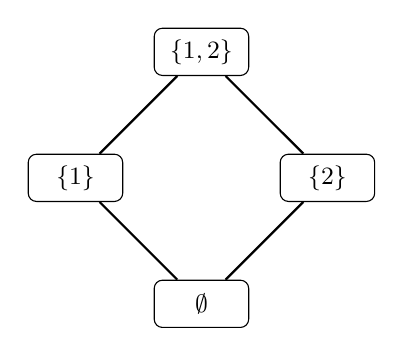
\begin{tikzpicture}[
        every node/.style={draw=black, rounded corners=3pt, minimum width=1.2cm, minimum height=0.6cm, inner sep=4pt, font=\small},
        scale=1.6
    ]
        \node (top) at (0,2) {$\{1, 2\}$};
        \node (a)   at (-1,1) {$\{1\}$};
        \node (b)   at (1,1) {$\{2\}$};
        \node (bot) at (0,0) {$\emptyset$};
    
        \draw[thick] (bot) -- (a);
        \draw[thick] (bot) -- (b);
        \draw[thick] (a) -- (top);
        \draw[thick] (b) -- (top);
    \end{tikzpicture}
    \caption{Reticolo completo dell'insieme delle parti $\mathcal{P}(\{1,2\})$ ordinato per inclusione ($\subseteq$); l'estremo inferiore $\bot$ è l'insieme vuoto $\emptyset$, mentre l'estremo superiore $\top$ è l'insieme completo}
\end{figure}

Avere un reticolo completo ci permette di enunciare due teoremi fondamentali che garantiscono l'esistenza (e la calcolabilità) dei punti fissi per le funzioni su questi domini (un valore $x$ è un \textit{punto fisso} per una funzione $f$ se $f(x) = x$).

\begin{defframe}{Teorema di Knaster-Tarski}{}
    In un reticolo completo $(L, \apprord)$, \textbf{ogni funzione monotona} ammette un massimo e un minimo punto fisso.
\end{defframe}

Il teorema di Knaster-Tarski assicura l'esistenza del punto fisso, ma non dice come trovarlo. Il teorema di Kleene ci fornisce invece un metodo costruttivo.

\begin{defframe}{Teorema di Kleene (del minimo punto fisso)}{}
    Se una funzione $f$ è \textbf{continua}, il suo minimo punto fisso (Least Fixed Point, LFP) può essere costruito iterativamente partendo dal livello minimo di informazione ($\bot$).
    
    Esso è definito come il limite delle applicazioni ripetute di $f$:
    \[ \text{LFP}(f) = f^\omega(\bot) = \lim_{n\to\infty} f^n(\bot) = \sqcup \{ \bot, f(\bot), f(f(\bot)), \dots \} \]
    \begin{proofframe}
    Sappiamo che la sequenza $\bot \apprord f(\bot) \apprord f(f(\bot)) \dots$ è una catena monotona crescente e che quindi (poiché ci troviamo in un CPO) ha un estremo superiore.

    Possiamo dimostrare che questo estremo superiore $f^\omega$ è un punto fisso sfruttando la continuità:
    \begin{align*}
        f^\omega &= \sup \{ f^i(\bot) \mid i < \omega \} \quad &\text{(per definizione di } f^\omega \text{)} \\
        &= \sup \{ f(f^i(\bot)) \mid i < \omega \} \quad &\text{(spostando l'indice di 1 passo)} \\
        &= f(\sup \{ f^i(\bot) \mid i < \omega \}) \quad &\text{(per la continuità di } f\text{)} \\
        &= f(f^\omega) \quad &\text{(sostituendo la definizione di } f^\omega\text{)}
    \end{align*}
    Poiché $f(f^\omega) = f^\omega$, $f^\omega$ è per definizione un punto fisso di $f$.
    \end{proofframe}
\end{defframe}

\begin{gframe}{Significato computazionale dei teoremi di punto fisso}
Quando scriviamo una definizione ricorsiva come \code{ones = 1 : ones}, stiamo implicitamente definendo un'equazione: $x = f(x)$, dove la funzione è $f(x) = 1 : x$ - stiamo quindi cercando il punto fisso di $f$.

Il Teorema di Kleene ci spiega esattamente cosa fa la valutazione lazy: il computer costruisce la lista infinita partendo dal non-calcolato ($\bot$) e applicando la funzione in modo continuo:
\begin{enumerate}
    \item $f^0(\bot) = \bot$ \hfill \textit{(nessuna informazione)}
    \item $f^1(\bot) = 1 : \bot$ \hfill \textit{(primo elemento noto)}
    \item $f^2(\bot) = 1 : 1 : \bot$ \hfill \textit{(secondo elemento noto)}
\end{enumerate}
Il limite di questo processo all'infinito ($f^\omega$) è proprio la nostra lista infinita. La continuità garantisce che per estrarre una quantità di informazione finita dall'output (es. \code{take 2 ones}), il computer debba compiere solo un numero finito di passi, senza bloccarsi cercando di valutare l'intera struttura infinita.
\end{gframe}

\section{Induzione e co-induzione}

Nella teoria dei tipi e nella programmazione funzionale, le strutture dati possono essere definite in due modi duali: tramite induzione (costruendo valori) o tramite co-induzione (osservando valori). Queste due visioni corrispondono alla ricerca di minimi e massimi punti fissi.

\begin{defframe}{Insiemi (Algebre) Induttivi}{}
    Un insieme \textbf{induttivo} $A$ viene definito "partendo dal basso" (tipicamente dall'insieme vuoto), definendo le regole (costruttori) che permettono di creare valori di tipo $A$.
    
    \begin{itemize}
        \item $A$ è il \textbf{minimo} insieme chiuso rispetto alle operazioni di costruzione (rappresentato da un assioma di minimalità, es. "nient'altro è un numero naturale");
        \item L'insieme $A$ rappresenta il \textbf{minimo punto fisso} di un'operazione di costruzione;
        \item Gli elementi di $A$ sono il risultato di un'applicazione \textbf{finita} dei costruttori, a partire da costruttori costanti.
            \item Da un punto di vista logico, ad $A$ è associato un \textbf{principio di induzione} per provare proposizioni su $A$.
            \item Da un punto di vista informatico (minima algebra / oggetto iniziale in Teoria delle Categorie), ad $A$ è associato un principio di \textbf{ricorsione e/o iterazione} (come \code{fold}) per definire funzioni che "consumano" il tipo: $f \colon A \to B$.
    \end{itemize}
\end{defframe}

\begin{defframe}{Insiemi (Co-algebre) Co-induttivi}{}
    Un insieme \textbf{co-induttivo} $A$ viene definito "partendo dall'alto" (ad esempio da un universo $U$), definendo le regole (distruttori) che permettono di riconoscere i valori che \textit{non} appartengono ad $A$.
    
    \begin{itemize}
        \item $A$ è il \textit{massimo} insieme chiuso rispetto alle operazioni di eliminazione. 
        \item L'insieme $A$ rappresenta il \textbf{massimo punto fisso} di un'operazione di eliminazione.
        \item Gli elementi scartati ($U \setminus A$) vengono riconosciuti dopo un numero finito di applicazioni dei distruttori, ma per gli elementi di $A$ questo processo può continuare all'infinito (es. liste infinite o stream).
            \item Da un punto di vista logico, ad $A$ è associato un \textbf{principio di co-induzione} (come la bisimulazione), usato solitamente per provare \textit{equivalenze} su $A$.
            \item Da un punto di vista informatico (massima algebra / oggetto finale in Teoria delle Categorie), ad $A$ è associato un principio di \textbf{co-ricorsione e/o co-iterazione} (come \code{unfold} o \code{iterate}) per definire funzioni che "generano" o costruiscono oggetti di tipo $A$: $f \colon B \to A$.
    \end{itemize}
\end{defframe}

\subsection{Insiemi induttivi (e relativi funzionali)}
\begin{gframe}{Approfondimento: lemma di Lambek}
        Se consideriamo l'algebra induttiva come un \textit{oggetto iniziale} nella Teoria delle Categorie, il principio di ricorsione in programmazione è l'incarnazione computazionale dell'\textbf{omomorfismo unico} definito dal Lemma di Lambek (vedi \href{https://raw.githubusercontent.com/AglaiaNorza/notes-ig/main/terzo%20anno/linguaggi%20di%20programmazione.pdf}{\underline{appunti del corso ``Linguaggi di programmazione''} })
    
    Definire una funzione ricorsiva $f \colon A \to B$ su un tipo induttivo $A$ significa costruire l'unico omomorfismo unico che mappa i costruttori di $A$ nelle operazioni di un'altra algebra $B$.
\end{gframe}

    Ogni tipo induttivo ha il proprio operatore fondamentale (un costrutto di ordine superiore) che si occupa di "costruire" questo omomorfismo:
    \begin{itemize}
    \item \textbf{Tipi ``non ricorsivi'' (Booleani, Either):} anche se raramente definiti come tipi ricorsivi, possiedono un principio di ricorsione. Per i booleani è semplicemente l'\code{if-then-else}, mentre per il tipo \code{Either} è l'applicazione di due funzioni $g$ e $h$ a seconda del costruttore (\code{Left} o \code{Right}). Il principio di induzione associato è l'analisi per casi.
        
        \item \textbf{Numeri naturali ($\mathbb{N}$):} l'operatore matematico che costruisce l'omomorfismo è \textbf{$\rho$ (iteratore)}. In Haskell, esso prende la forma della funzione \code{iter}:
        \begin{haskellbox}{}
iter f b 0 = b
iter f b n = f (iter f b (n-1))
\end{haskellbox}

        Questo comportamento ricalca esattamente la semantica dei \textbf{Numerali di Church}. 

Per ottenere una potenza espressiva maggiore, si passa allo schema della \textit{ricorsione primitiva} (l'operatore \code{rec}), in cui la funzione $f$ riceve in input anche il contatore $(n-1)$:

\begin{haskellbox}{}
rec f b 0 = b
rec f b n = f (n-1) (rec f b (n-1))
\end{haskellbox}

(rec permette di definire facilmente funzioni il cui risultato dipende sia dal risultato del passo ricorsione precedente, che dal ``contatore''; per esempio, il fattoriale:
\begin{haskellbox}{}
    -- f prende il contatore e il risultato della ricorsione
factorial n = rec (\cont res -> (cont + 1) * res) 1 n
    -- fattoriale di n = n (ovvero contatore+1) * fattoriale (n-1) (passo prec)
\end{haskellbox}
)
        
        \item \textbf{Liste finite:} sulle liste l'operazione che costruisce l'omomorfismo "sostituendo" i costruttori della lista con operazioni su un altro tipo è la \code{foldr}. Rappresenta il principio di iterazione/ricorsione generalizzato per le liste:
    \begin{haskellbox}{}
iter f b [] = b
iter f b (x:xs) = f x (iter f b xs)  -- corrisponde a foldr f b xs
    \end{haskellbox}
    \end{itemize}

\subsection{Insiemi coinduttivi (e relativi funzionali)}
L'insieme coinduttivo che origina dai costruttori dei numeri naturali è formato dai naturali, più un \textbf{naturale infinito non-standard} $\omega = S^{\infty}$, ottenuto da infinite applicazioni del costruttore $S$.

L'insieme coinduttivo più interessante è quello delle liste infinite (o \textbf{Stream}). Non ha senso definire funzioni per ricorsione su di esse, ma si possono sempre definire funzioni che creano Stream di cui, in tempo finito, si può accedere ad una porzione finita.

Il principio di ricorsione sulle Stream si può definire tramite due funzionali:
\begin{itemize}
    \item \code{iterate}, che permette di definire una funzione \code{f :: a -> Stream b}
        \subitem data una funzione \code{f :: a -> b } ed un valore \code{x :: b}, permette di costruire uno stream in questo modo:
        \begin{haskellbox}{}
iterate f x = x : iterate f (f x)
        \end{haskellbox}

        (crea quindi lo stream \code{x : f x : f (f x) : ... })
\end{itemize}

Conviene però avere un principio di ricorsione più generale: la cosiddetta \textbf{co-ricorsione}, ottenibile con il funzionale \code{unfold}.

\begin{haskellbox}{}
unfold :: (b -> (a, b)) -> b -> Stream a
unfold f y = x : unfold f y' where (x, y') = f y
\end{haskellbox}

Il funzionale \code{unfold} può essere visto come un \textbf{generatore infinito} regolato da una macchina a stati.

Consideriamo la firma del suo tipo:
\[ \code{unfold} :: (b \to (a, b)) \to b \to \text{Stream } a \]

\begin{itemize}
    \item \textbf{Il tipo $b$ (seme o stato interno)} rappresenta l'informazione corrente necessaria e sufficiente per calcolare il prossimo elemento dello stream.
    \item \textbf{La funzione $f :: b \to (a, b)$ (generatore)} ``apre'' (da cui \textit{unfold}) lo stato attuale $y$ per produrre una coppia $(x, y')$, in cui:
    \begin{itemize}
        \item $x$ (di tipo $a$) è il \textbf{valore} effettivo che viene emesso in output ed entra a far parte dello Stream
        \item $y'$ (di tipo $b$) è il \textbf{nuovo seme} che verrà riutilizzato come argomento al passo successivo della computazione
    \end{itemize}
\end{itemize}

A ogni iterazione, il funzionale prende lo stato corrente, produce un elemento visibile all'esterno e aggiorna lo stato interno per la computazione futura, ``srotolando'' il seme iniziale all'infinito.

\begin{gframe}{Produttività}
Nelle strutture dati infinite, il concetto classico di \textit{terminazione} perde di significato (lo stream, per definizione, non deve mai finire). Al suo posto, si introduce il criterio di \textbf{produttività}:
\begin{quote}
    Una funzione co-ricorsiva si dice \textbf{produttiva} se è in grado di valutare una qualsiasi porzione finita del suo output (ad esempio l'elemento di testa) in un \textbf{tempo finito}.
\end{quote}

Nel codice di \code{unfold}, la produttività è garantita dal costruttore di lista (\code{:}). Poiché il costruttore si trova all'esterno della chiamata co-ricorsiva (\code{x : unfold f y'}), Haskell può istanziare immediatamente la testa \code{x} e congelare la computazione del resto dello stream (\code{unfold f y'}) sotto forma di \textit{thunk}, finché non sarà esplicitamente richiesta da una successiva operazione di accesso.
\end{gframe}

Possiamo ridefinire il funzionale \code{iterate} precedentemente analizzato come un caso particolare di co-ricorsione in cui lo stato interno e il tipo dell'elemento emesso coincidono ($a = b$):
\begin{haskellbox}{}
iterate :: (a -> a) -> a -> Stream a
iterate f x = unfold (\s -> (s, f s)) x
\end{haskellbox}
In questo caso, il generatore prende lo stato \code{s}, lo restituisce come elemento corrente dello stream e applica \code{f s} per determinare il nuovo seme per il passo successivo.

Se invece vogliamo considerare l'algebra che contiene la lista vuota, allora la massima co-algebra contiene anche le liste finite. In tal caso, possiamo definire il funzionale \code{unfoldLS}, che costruisce anche liste finite:
\begin{haskellbox}{}
unfold :: (b -> Bool) -> (b -> (a, b)) -> b -> [a]
unfold p f y = if p y then []
            else x : unfold p f y' where (x, y') = f y
\end{haskellbox}

\subsection{Bisimulazione}
Come per gli insiemi induttivi, abbiamo bisogno di un modo per derivare equivalenze su insiemi co-iduttivi. La controparte dell'induzione che ci permette di farlo è la \textbf{bisimulazione}.

L'idea alla base della bisimulazione è osservare se due processi (o liste) ``si comportano'' allo stesso modo per ogni osservazione finita che possiamo farne.

Si procede in questo modo:
\begin{enumerate}
    \item si definisce una relazione $R$ tra due liste
    \item se si dimostra che per ogni coppia $(xs, ys) \in R$, le loro teste sono uguali e le loro code sono ancora in $R$, allora le liste si dicono \textbf{bisimili} ($\approx$)
\end{enumerate}

Formalmente, si definisce una bisimulazione $R$ tra coppie di liste come segue:
\begin{align*}
    R \ xs \ ys \implies & xs = ys = \bot \text{ oppure } xs = ys = [ \ ] \\
                         & \text{oppure } \exists v, vs, ws \text{ t.c. } xs = v:vs \land ys = v:ws \land vs \ R \ ws
\end{align*}

Definiamo quindi $xs \approx ys$ se esiste una bisimulazione $R$ tale che $xs \ R \ ys$, il che equivale a scegliere la \textbf{massima equivalenza}, definita come massimo punto fisso.

\begin{gframe}{Prova per bisimulazione}
    Possiamo dimostrare per bisimulazione che:
    \begin{haskellbox}{}
map f (iterate f x) = iterate f (f x)
    \end{haskellbox}
    Ci basta dimostrare che la relazione $R$ che contiene:
    $$\{ \code{map f (iterate f x), iterate f (f x)} \mid \code{f,x} \text{ opportuni} \}$$
    è una bisimulazione.

    Facendo ricorso all'algebra dei programmi, possiamo ``svolgere'' le due espressioni:
    \begin{haskellbox}{}
map f (iterate f x) = map f (x : iterate f (f x))
                    = f x : map f (iterate f (f x))

    \end{haskellbox}
e anche
    \begin{haskellbox}{}
iterate f (f x) = f x : iterate f (f (f x))
    \end{haskellbox}

    Entrambe producono la stessa testa (\code{f x}), e le code sono in $R$ (in cui la nuova funzione applicata sarà \code{f.f} invece di \code{f}).
\end{gframe}

\subsection{Dimostrazione per approssimazione}
L'alternativa alla co-induzione consiste nell'effettuare una dimostrazione per induzione sulle approssimazioni finite di una lista. Per farlo, si internalizza in Haskell la funzione \code{approx}, strettamente imparentata con \code{take}:

\begin{haskellbox}{}
approx 0 xs = undefined
approx n [] = []
approx n (x:xs) = x : approx (n-1) xs
\end{haskellbox}

La proprietà fondamentale di \code{approx} è che il limite delle approssimazioni di una lista è la lista stessa:
$$\sqcup_{n} \text{approx } n \ xs = xs$$

Di conseguenza, per dimostrare l'uguaglianza tra due liste $xs$ e $ys$, è sufficiente mostrare che tutte le loro approssimazioni finite siano uguali per ogni $n$:
$$\forall n, \text{approx } n \ xs = \text{approx } n \ ys \implies xs = ys$$

\begin{gframe}{Esempio}
Proviamo a dimostrare nuovamente la proprietà:
$$\text{approx } n \ (\text{map } f \ (\text{iterate } f \ x)) = \text{approx } n \ (\text{iterate } f \ (f \ x))$$

\begin{itemize}
    \item \textbf{caso base:} per $n = 0$ la proprietà è banalmente vera perché \code{approx 0 xs} restituisce sempre $\perp$ (undefined).

    \item \textbf{caso induttivo:} si procede riducendo le due espressioni separatamente tramite program calculation e applicando l'ipotesi induttiva:

\begin{align*}
    & \text{approx } (n+1) \ (\text{iterate } f \ (f \ x)) \\
    = & \{ \text{def. di iterate} \} \\
    & \text{approx } (n+1) \ (f \ x : \text{iterate } f \ (f \ (f \ x))) \\
    = & \{ \text{def. di approx} \} \\
    & f \ x : \text{approx } n \ (\text{iterate } f \ (f \ (f \ x))) \\
    = & \{ \text{ipotesi induttiva} \} \\
    & f \ x : \text{approx } n \ (\text{map } f \ (\text{iterate } f \ (f \ x))) \\
    = & \{ \text{def. di approx al contrario} \} \\
    & \text{approx } (n+1) \ (f \ x : \text{map } f \ (\text{iterate } f \ (f \ x))) \\
    = & \{ \text{def. di map al contrario} \} \\
    & \text{approx } (n+1) \ (\text{map } f \ (x : \text{iterate } f \ (f \ x))) \\
    = & \{ \text{def. di iterate al contrario} \} \\
    & \text{approx } (n+1) \ (\text{map } f \ (\text{iterate } f \ x))
\end{align*}
\end{itemize}
\end{gframe}

\section{Funtori e Applicativi}

\begin{gframe}{Concetti principali}
    Sia i Funtori che gli Applicativi servono a gestire computazioni all'interno di un \textbf{contesto}, ma con ``poteri'' diversi:
    \begin{itemize}
        \item \textbf{Functors}: permettono di applicare una funzione "pura" a un valore nel contesto - modificano il contenuto ma non la struttura del contesto;
        \item \textbf{Applicatives}: permettono di applicare funzioni che sono esse stesse dentro un contesto a valori nel contesto - sono necessari per gestire funzioni con più argomenti;
    \end{itemize}
\end{gframe}

\begin{center}
\begin{tabular}{|l|l|l|}
\hline
\textbf{classe} & \textbf{operatore} & \textbf{scopo} \\ \hline
\code{Functor} & \code{fmap :: (a -> b) -> t a -> t b} & trasformazione (1 argomento) \\ \hline
\code{Applicative} & \code{<*> :: t (a -> b) -> t a -> t b} & combinazione ($n$ argomenti) \\ \hline
\end{tabular}
\end{center}

\subsection{Funtori}

L'idea alla base di un \textbf{funtore} è la generalizzazione del funzionale \code{map}, tipicamente utilizzato per le liste, a tutti i possibili costruttori di tipo.

Se si ha:
\begin{itemize}
    \item una funzione $f:: a\to b$
    \item un costruttore di tipo $T$ che trasforma un tipo $a$ in un tipo $t a$ (come per esempio \code{[a]} oppure \code{Maybe a})
\end{itemize}

Si può ottenere in modo canonico una funzione
$$T f :: t a \to t b$$

\begin{center}
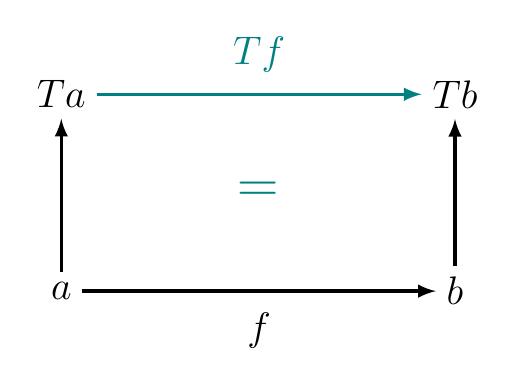
\begin{tikzpicture}[x=5cm, y=2.5cm, >=latex, very thick, font=\Large]
    \node (a)  at (0,0) {$a$};
    \node (b)  at (1,0) {$b$};
    \node (Ta) at (0,1) {$Ta$};
    \node (Tb) at (1,1) {$Tb$};
    
    \node[text=teal] at (0.5, 0.5) {\huge $\mathbf{=}$};
    
    \draw[->] (a) -- node[below=4pt] {$f$} (b);
    \draw[->] (a) -- (Ta);
    \draw[->] (b) -- (Tb);
    
    \draw[->, teal] (Ta) -- node[above=4pt, text=teal] {$Tf$} (Tb);
\end{tikzpicture}
\end{center}

\begin{gframe}{}
Nel mondo categoriale, il concetto di ``funtore'' descrive un passaggio tra due categorie: dati due oggetti (tipi come $a$ o $b$), un funtore agisce come un costruttore di tipo ($T$) - prende un oggetto $a$ nella categoria $C$ e lo trasforma in un oggetto $t a$ nella categoria $D$.
\begin{itemize}
    \item il punto importante è che un funtore non mappa solo i tipi, ma anche le relazioni tra essi: se esiste una funzione $f : a \to b$, il funtore deve fornire un modo per ottenere una funzione corrispondente $t f$ che operi sui tipi $t a \to t b$
    \item un funtore è quindi una \textbf{mappa che preserva la struttura}
\end{itemize}
\end{gframe}

La classe \code{Functor} richiede che sia definita una funzione \code{fmap}, che rende commutativo il passaggio dai tipi base ai tipi ``inscatolati''

\begin{haskellbox}{}
class Functor t where
    fmap :: (a -> b) -> t a -> t b
\end{haskellbox}
\begin{itemize}
    \item il tipo di \code{fmap} è parametrico, oltre che nei tipi \code{a} e \code{b}, anche rispetto a un \textbf{costruttore di tipo} \code{t} (si vede che \code{t} deve essere un costruttore di tipo perché si applica ad altri tipi)
\end{itemize}

\code{fmap} prende quindi una funzione \code{a -> b} e un valore ``inscatolato'' \code{t a}, e :
\begin{itemize}
    \item ``spacchetta'' il valore
    \item applica la funzione
    \item ``impacchetta'' il risultato
\end{itemize}

\begin{center}
    \includegraphics[width=3cm]{assets/ouch}
\end{center}

\begin{center}
\includegraphics[width=9cm]{assets/fmap_apply}
\end{center}
\vspace{-1em}
(immagini prese da \href{https://www.adit.io/posts/2013-04-17-functors,_applicatives,_and_monads_in_pictures.html}{qui} !!)

\begin{gframe}{Esempi}
    Alcuni esempi noti di istanze di funtori sono:
    \begin{itemize}
        \item le liste
\begin{haskellbox}{}
instance Functor [] where
    fmap = map
\end{haskellbox}

\item il tipo \code{Maybe}
\begin{haskellbox}{}
instance Functor Maybe where
    fmap f Nothing = Nothing
    fmap f (Just x) = Just (f x)
\end{haskellbox}
\end{itemize}

\begin{center}
\includegraphics[width=13cm]{assets/fmap_just}
\end{center}

\end{gframe}

Possiamo definire i funtori anche per esempio sugli alberi binari:
\begin{haskellbox}{}
instance Functor BinTree where
    fmap f (Leaf x) = Leaf (f x)
    fmap f (Branch l r) = Branch (fmap f l) (fmap f r)
\end{haskellbox}

Definire un tipo come istanza di \code{Functor} permette di scrivere codice generico che funziona su diverse strutture dato. 

Per esempio, si può definire una funzione \code{inc} che incrementa i valori all'interno di qualsiasi funtore:
\begin{haskellbox}{}
inc :: Functor t => t Int -> t Int
inc = fmap (+1)
\end{haskellbox}

\subsubsection{Funzioni come funtori}
Un'estensione interessante del concetto di funtore si ha quando consideriamo le \textbf{funzioni stesse} come istanze della classe \code{Functor}.

In questo caso, il costruttore di tipo è l'operatore freccia parzialmente applicato, ovvero \code{((->) r)}. Questo costruttore prende un tipo $a$ e lo trasforma nel tipo di una funzione che si aspetta un input di tipo $r$, cioè \code{r -> a}. 

Se proviamo a sostituire il costruttore \code{t} con \code{((->) r)} nella firma di \code{fmap}, otteniamo:
\begin{center}
    \code{fmap :: (a -> b) -> ((->) r a) -> ((->) r b)}
\end{center}

Che riscritta in forma infissa diventa:
$$ \code{fmap :: (a -> b) -> (r -> a) -> (r -> b)} $$

Questa firma coincide con quella dell'operatore di \textbf{composizione di funzioni} (\code{.}). Di conseguenza, l'istanza si definisce semplicemente così:
\begin{haskellbox}{}
instance Functor ((->) r) where
    fmap f g = f . g
    -- o in forma contratta: fmap = (.)
\end{haskellbox}

\begin{gframe}{Intuizione}
L'idea di "contenitore" qui sfuma in quella di \textbf{contesto computazionale}:
\begin{itemize}
    \item un valore di tipo \code{r -> a} può essere visto come una scatola che non contiene ancora un valore di tipo $a$, ma sa come produrlo non appena le viene fornito un input di tipo $r$
    \item applicare \code{fmap f g} significa post-elaborare il risultato della computazione: non appena \code{g} produrrà il suo valore di tipo $a$, questo verrà immediatamente passato a \code{f} per ottenere un tipo $b$
\end{itemize}
\end{gframe}

Grazie a questa proprietà, mappare una funzione sopra un'altra significa semplicemente creare una pipeline logica in cui il flusso dei dati attraversa le funzioni in sequenza.

\begin{center}
\includegraphics[width=7cm]{assets/fmap_function}
\end{center}

\subsubsection{Functor laws}
Affinché un funtore sia definito correttamente, è necessario che rispetti le due functor laws:
\begin{enumerate}
    \item \code{fmap id = id}
    \item \code{fmap (f . g) = fmap f . fmap g}
\end{enumerate}

Nota bene: queste leggi non possono essere verificate dal type-checker, ma sono responsabilità del programmatore Haskell !

\begin{gframe}{Funtori come omomorfismi}
    Possiamo notare, osservando le \textit{functor laws}, che un funtore è effettivamente un \textbf{omomorfismo tra categorie} (un omomorfismo ``classico'' preserva l'operazione di gruppo, mentre un funtore preserva la ``struttura'' di una categoria, ovvero gli oggetti - i tipi -, e i morfismi - le funzioni.)
\end{gframe}

\subsubsection{Notazione infissa}
Il modulo \code{Data.Functor} definisce anche una notazione alternativa per \code{fmap}: la sua versione infissa, \code{<\$>}.
\begin{haskellbox}{}
(<$>) :: Functor t => (a -> b) -> t a -> t b
f <$> x = fmap f x

-- (+1) <$> [1, 2, 3] ->  [2, 3, 4]
\end{haskellbox}

\subsubsection{Lifting}
Come abbiamo visto all'inizio di questa sezione, un modo di vedere \code{fmap} è attraverso il \textit{currying} del suo tipo. Cambiando l'ordine concettuale delle parentesi nella segnatura:
$$\code{fmap :: (a -> b) -> (t a -> t b)}$$
In quest'ottica, \code{fmap} prende una funzione normale $a \to b$ e la \textbf{solleva} nel mondo dei contesti, trasformandola in una funzione tra strutture $t a \to t b$. Per questo motivo, a volte in Haskell si trova la funzione storica \code{liftM} (o simili), che concettualmente fa la stessa cosa.

\subsubsection{Il limite dei Funtori: funzioni multi-argomento}
Cosa succede se proviamo a mappare una funzione che accetta due o più argomenti (come l'addizione \code{(+) :: Int -> Int -> Int}) su un funtore?

Se valutiamo:
\begin{haskellbox}{}
(+) <$> Just 3
\end{haskellbox}
Ricordando che in Haskell tutte le funzioni sono curryficate, \code{(+)} applicata a $3$ restituisce una funzione parziale \code{(3+)}. Di conseguenza, il tipo del risultato sarà:
\begin{haskellbox}{}
Just (3+) :: Maybe (Int -> Int)
\end{haskellbox}

Abbiamo ottenuto una funzione inscatolata nel contesto. Il limite di \code{Functor} sta nel fatto che con \code{fmap} non abbiamo alcun modo di applicare questa funzione \code{Maybe (Int -> Int)} a un altro valore anch'esso dentro un \code{Maybe} (ad esempio \code{Just 5}).

\subsection{Applicativi}
Un normale funtore permette di usare \code{fmap} con un solo argomento, ma è naturale voler generalizzare: si vuole considerare una forma astratta di applicazione, che generalizzi l'usuale applicazione di funzioni. Per esempio, si vuole poter propagare un fallimento nel caso di \code{Maybe}, o applicare una funzione $n$-aria a valori ``inscatolati'' senza dover istanziare $n$ funtori.

Haskell definisce quindi la classe \code{Applicative}.

\begin{haskellbox}{}
class Functor t => Applicative t where
    pure :: a -> t a
    (<*>) :: t (a -> b) -> t a -> t b
\end{haskellbox}

Un applicativo estende un funtore, e richiede due operatori fondamentali:
\begin{itemize}
    \item \code{pure}: prende un valore ``normale'' e lo immerge nel contesto (lo ``impacchetta'')
        \subitem per esempio, per \code{Maybe}, \code{pure x} è \code{Just x}
    \item \code{<*>} (\textit{splat} o \textit{apply}): prende una funzione ``impacchettata'' in un contesto (\code{t (a -> b)}) e un valore anch'esso in un contesto (\code{t a}), ``scarta'' concettualmente entrambi i contesti, applica la funzione al valore (gestendo gli effetti del contesto), produce il risultato e lo ``incarta'' nel contesto (\code{t b})
\end{itemize}

\begin{center}
    \includegraphics[width=12cm]{assets/applicative_just}
\end{center}

Possiamo istanziare \code{Maybe} anche come applicativo:
\begin{haskellbox}{}
instance Applicative Maybe where
    pure = Just
    Nothing <*> _ = Nothing -- se uno dei due è Nothing, entrambi sono Nothing

    -- potremmo fare 
    -- Just f <*> Just x = Just (f x) ma abbiamo già fmap dei Funtori !
    -- se "spacchettiamo" f e non x, otteniamo esattamente la segnatura
    -- dei funtori (a->b) -> f a e possiamo fare:

    (Just f) <*> mx = fmap f mx
    -- <*> prende quindi una funzione e un valore in un contesto
    -- per es. Just (+3) <*> Just 2 = Just 5
\end{haskellbox}


\begin{gframe}{Combinare \code{<\$>} e \code{<*>}: stile applicativo}
\begin{haskellbox}{}
(*) <$> (Just 8) <*> (Just 2)
-- valuta a Just 16 !
\end{haskellbox}

Questo esempio mostra come combinare \code{fmap} (\code{<\$>}) e \code{<*>}:
\begin{itemize}
    \item l'operatore \code{<\$>} (fmap) prende la funzione binaria ``pura'' \code{(*)} e la mappa sul primo argomento contestualizzato \code{(Just 8)}; questo produce una funzione parzialmente applicata dentro il contesto: \code{Just (8 *)}.
    \item poiché ora la funzione è ``impacchettata'' nel contesto \code{Maybe}, non possiamo più usare un normale \code{fmap} per passarle il secondo argomento
    \item usiamo quindi \code{<*>}, che prende la funzione nel contesto \code{Just (8 *)}, la applica al valore nel contesto \code{(Just 2)} e propaga l'effetto, restituendo \code{Just 16}
\end{itemize}

Questo pattern si estende a funzioni con quanti argomenti si desidera, alternando sempre un \code{<\$>} iniziale e una catena di \code{<*>}:
\begin{haskellbox}{}
f <$> arg1 <*> arg2 <*> arg3 <*> ... <*> argN
\end{haskellbox}

Teoricamente, potremmo anche scrivere \code{pure (*) <*> Just 8 <*> Just 2}.

Tipicamente, si scriverebbe in quel modo per mostrare didatticamente come \code{<*>} lavori sempre su due strutture dello stesso tipo. Nel codice reale, tuttavia, si preferisce iniziare con \code{<\$>} grazie a una legge di equivalenza fondamentale degli applicativi:
\begin{haskellbox}{}
pure f <*> x  ==  f <$> x
\end{haskellbox}
Usare \code{<\$>} all'inizio è la scelta più idiomatica perché evita di dover ``impacchettare'' artificialmente la funzione per poi doverla subito combinare col primo argomento.

L'operatore \code{pure} resta comunque indispensabile in due scenari principali:
\begin{itemize}
    \item inserire valori costanti a metà catena: se una funzione richiede tre argomenti, di cui i primi due contestualizzati e il terzo fisso, usiamo \code{pure} per iniettarlo senza rompere la catena: 
        \subitem \code{f <\$> magariA <*> magariB <*> pure "valore\_fisso"}
    \item incartare un valore singolo: quando si vuole semplicemente inserire un valore in un contesto senza applicargli alcuna funzione (es. \code{pure 5 :: [Int]} produce \code{[5]}).
\end{itemize}

\end{gframe}

\subsubsection{Liste come applicativi}
L'istanza del Prelude delle liste non si comporta come una \code{zipWith} nell'applicare le funzioni presenti in una lista, ma modella un non-determinismo. Una lista non viene vista come una sequenza, ma come un valore che può assumere più risultati posssibili contemporaneamente. Quindi, quando si applica una lista di funzioni ad una lista di valori, l'applicativo contiene tutte le combinazioni possibili (prodotto cartesiano).

\begin{center}
\includegraphics[width=10cm]{assets/applicative_list}
\end{center}

\begin{haskellbox}{}
instance Applicative [] where
    -- pure : a -> [a]
    pure x = [x]

    -- <*> : [a -> b] -> [a] -> [b]
    fs <*> xs = [f x | f <- fs, x <- xs]
    -- ^ prodotto cartesiano 
\end{haskellbox}

Se eseguiamo quindi \code{pure (*) <*> [1,2] <*> [3,4]} (o, in stile applicativo, \\
\code{(*) <\$> [1,2] <*> [3,4]}):
\begin{itemize}
    \item \code{pure (*)} crea \code{[(*)]}
    \item \code{[(*)] <*> [1,2]} produce una lista di funzioni \code{[(1*), (2*)]}
    \item \code{[(1*), (2*)] <*> [3,4]} applica entrambe le funzioni ad entrambi i numeri
        \subitem si ottiene quindi \code{1*3, 1*4, 2*3, 2*4} $\to$ \code{[3, 4, 6, 8]}
\end{itemize}

A volte si vuole però che le liste si comportino come \code{zipWith} - per questo, Haskell introduce \code{ZipList}

\begin{haskellbox}{}
 -- per poter definire un'altra istanza di Applicative senza conflitti
newtype ZipList a = Z [a]

instance Applicative ZipList where
    -- pure : a -> ZipList a
    pure x = Z (repeat x) -- crea una lista infinita di x

    -- <*> : [a -> b] -> [a] -> [b]
    Z fs <*> Z xs = Z (zipWith (\f x -> f x) fs xs)
\end{haskellbox}

\begin{itemize}
    \item \code{pure} è \code{repeat} così che si adatti a qualsiasi lunghezza della lista di valori con cui verrà  accoppiata (se restituisse un solo elemento, \code{zipWith} si fermerebbe subito)
    \item \code{<*>} è \code{zipWith} - applica la funzione in posizione 1 al valore in posizione 1 ecc
\end{itemize}

\subsubsection{Esempio: alberi come applicativi}
Consideriamo una struttura dati ad albero binario definito sulle foglie:
\begin{haskellbox}{}
data BinTree a = Leaf a | Branch (BinTree a) (BinTree a)

instance Functor BinTree where
    fmap f (Leaf x) = Leaf (f x)
    fmap f (Branch l r) = Branch (fmap f l) (fmap f r)
\end{haskellbox}

Come per le liste, esistono due modi concettualmente diversi di estendere questa struttura ad un \code{Applicative}.

\paragraph{1. L'approccio zip-like}
Il primo modo consiste nell'applicare le funzioni ai nodi corrispondenti per posizione, fondendo le strutture (come per \code{ZipList}). 

In questo caso, \code{pure} genera un albero infinito composto dalla stessa foglia, in modo da potersi "adattare" a qualsiasi forma dell'albero a cui verrà applicato.

\begin{haskellbox}{}
instance Applicative BinTree where
    -- pure crea una foglia che si espande virtualmente all'infinito
    pure x = Leaf x

    -- <*> applica le funzioni ricorsivamente mantenendo la struttura
    -- caso base: applico la funzione alla foglia
    (Leaf f) <*> (Leaf x) = Leaf (f x)
    -- abbiamo una funzione in una foglia ma un branch a cui applicarla;
    -- si "duplica" la funzione e si applica sia a dx che a sx
    (Leaf f) <*> (Branch l r) = Branch (fmap f l) (fmap f r)
    -- per far combaciare le strutture, "copiamo" la foglia
    (Branch l r) <*> (Leaf x) = Branch (l <*> Leaf x) (r <*> Leaf x)
    -- la parte sinistra va a sinistra e quella destra a destra
    (Branch l r) <*> (Branch a b) = Branch (l <*> a) (r <*> b)
\end{haskellbox}

\paragraph{2. L'approccio combinatorio}
Se invece vogliamo che l'albero si comporti in modo "non-deterministico" (come l'istanza standard delle liste), ogni ramo dell'albero delle funzioni deve combinarsi con \textit{tutto} l'albero dei valori. Questo approccio potrebbe essere utile per clonare la struttura sotto una nuova radice comune.

\begin{gframe}{Esempio: Duplicare un albero con nuove radici}
    Immaginiamo di definire l'applicazione in modo che un albero di funzioni si distribuisca interamente sull'albero dei valori:
    \begin{haskellbox}{}
(Leaf f) <*> albero = fmap f albero
(Branch l r) <*> albero = Branch (l <*> albero) (r <*> albero)
    \end{haskellbox}

    Se ora creiamo un albero contenente delle funzioni parziali, ad esempio \\
    \code{Branch (Leaf (+2)) (Leaf (+3))}, e lo applichiamo tramite \code{<*>} ad un albero generico, otteniamo:
    
    \begin{haskellbox}{}
Branch (Leaf (+2)) (Leaf (+3)) <*> albero
-- Produce un unico albero avente come radice un Branch:
-- il sottoalbero sinistro sarà il vecchio albero con tutti i valori modificati da (+2),
-- il sottoalbero destro sarà il vecchio albero con tutti i valori modificati da (+3).
    \end{haskellbox}

In alternativa, senza riscrivere l'istanza di \code{Applicative}, lo stesso risultato si può ottenere combinando il costruttore \code{Branch} con \code{fmap} (\code{<\$>}) e \code{<*>}:
\begin{haskellbox}{}
nuovoAlbero = Branch <$> (fmap (+2) albero) <*> (fmap (+3) albero)
\end{haskellbox}
\end{gframe}


\subsubsection{Applicative laws}
Come i funtori, anche gli applicatori hanno una serie di regole da rispettare:
\begin{enumerate}
    \item \code{<*>} \textbf{preserva l'identità} 
        \subitem \code{pure id <*> x = x}
        \subitem se prendiamo la funzione identità, la inseriamo in un contesto e la applichiamo ad un valore \code{x} già contestualizzato, il risultato deve rimanere \code{x}
    \item \code{<*>} \textbf{preserva l'applicazione di funzioni}
        \subitem \code{pure (g x) = pure g <*> pure x}
        \subitem applicare \code{g} ad un valore \code{x} e poi ``impacchettare'' il risultato dà lo stesso esito che applicare la versione ``impacchettata'' di \code{g} alla versione ``impacchettata'' di \code{x}
    \item \textbf{non conta l'ordine} con cui si fa embedding nel contesto
        \subitem \code{f <*> pure y = pure (\textbackslash g -> g y) <*> f}
        \subitem applicare una funzione nel contesto \code{f} a un valore puro \code{y} equivale a invertire i ruoli: passare \code{f} come argomento a una struttura ``impacchettata'' (una lambda che aspetta una funzione) che contiene già il valore \code{y}
    \item \textbf{composizione} di \code{<*>}
        \subitem \code{f <*> (g <*> x) = (pure (.) <*> f <*> g) <*> x}
        \subitem (forma di associatività per \code{<*>})
        \subitem la composizione di funzioni \code{(.)} può essere ``lifted'' a livello applicativo per garantire che la sequenza delle applicazioni sia coerente
\begin{itemize}
    \item ovvero, applicare due funzioni una dopo l'altra è identico a comporle prima in un'unica funzione e poi applicarla:
        \subitem \code{f <*> (g <*> x)}
        \subitem prima si applica la funzione \code{g} al valore \code{x} (ottenendo un risultato nel contesto), e poi si applica \code{f} a tale risultato - è quindi \code{f(g(x))}
    \subitem \code{(pure (.) <*> f <*> g) <*> x}
\subitem qui l'operatore di composizione standard \code{(.)} viene ``sollevato'' (lifted) nel contesto, permettendo di fondere le due funzioni \code{f} e \code{g} dentro il contesto - si crea quindi una funzione composta che sarà applicata a \code{x}
\subitem quindi, si applica \code{f . g} a \code{x}, ottenendo anche qui \code{f(g(x))}
\end{itemize}
\end{enumerate}

\section{Monadi Base}
Le monadi rappresentano il passo successivo rispetto agli applicativi per la gestione controllata di \textbf{side-effects}. Se un applicativo permette di combinare calcoli indipendenti, la monade permette di gestire calcoli in cui il passo successivo \textbf{dipende} dal risultato di quello precedente.

\subsection{Introduzione}
Per comprendere perché le monadi siano utili, consideriamo un valutatore di espressioni aritmetiche che supporta costanti e divisioni:

\begin{haskellbox}{}
data Term = Const Int | Div Term Term

eval :: Term -> Int
eval (Const a) = a
eval (Div t u) = eval t `div` eval u
\end{haskellbox}

Questa implementazione è elegante ma fragile: un'espressione come \code{Div (Const 1) (Const 0)} farà crashare il programma.

Si può usare il tipo \code{Maybe Int} per modellare il possibile fallimento. Tuttavia, il codice diventa immediatamente prolisso a causa della propagazione manuale dell'errore:

\begin{haskellbox}{}
eval :: Term -> Maybe Int
eval (Const a) = Just a
eval (Div t u) = case eval t of
                   Nothing -> Nothing
                   Just n  -> case eval u of
                                Nothing -> Nothing
                                Just m  -> if m == 0 then Nothing 
                                           else Just (n `div` m)
\end{haskellbox}

La divisione (il vero senso della funzione) è offuscata dalla gestione dei \code{Nothing}.

Si potrebbe pensare di usare l'operatore \code{<*>} degli applicativi per pulire il codice. Tuttavia, gli applicativi sono insufficienti quando la struttura del calcolo dipende dal valore dei risultati intermedi:

\begin{itemize}
    \item L'operatore \code{<*>} (\code{f (a -> b) -> f a -> f b}) richiede che la funzione da applicare sia "pura" e che i contesti (\code{f}) siano già definiti. In un calcolo applicativo, l'intera sequenza di effetti è determinata a priori: non si può usare il valore estratto da un \code{Maybe} per decidere quale sarà il prossimo "effetto".
    
    \item Se provassimo a usare una funzione che genera essa stessa un contesto, come 

        \code{safeDiv :: Int -> Int -> Maybe Int}, l'applicazione risulterebbe in un tipo

        \code{Maybe (Maybe Int)}. 
    \begin{itemize}
        \item e.g. \code{pure safeDiv <*> Just 10 <*> Just 0} produce \code{Just (Nothing)}
    \end{itemize}
    L'applicativo non possiede un meccanismo per ``appiattire'' questi due livelli di contesto in uno solo.
    
\end{itemize}
 Nella divisione, il fatto che il secondo argomento sia zero determina se il calcolo successivo deve fallire o meno. In Haskell, questa capacità di far sì che il ``guscio'' esterno (il contesto) venga generato dal valore contenuto nel passo precedente è l'essenza delle Monadi.

    In sintesi: gli Applicativi modellano calcoli indipendenti (i contesti sono paralleli), mentre le Monadi (come ora vedremo) modellano calcoli sequenziali, dove il risultato di un'operazione influenza la creazione della successiva.

\begin{gframe}{}
In termini di Teoria delle Categorie, l'applicativo gestisce contesti indipendenti (funtori monoidali), mentre per concatenare funzioni del tipo $A \to M(B)$ (chiamate frecce di Kleisli) abbiamo bisogno di una Monade.
\end{gframe}

\subsection{Monadi (shall I be pure or impure?)}
Molti aspetti della programmazione (come strutture dati mutabili e input/output) non hanno una rappresentazione efficace nel mondo funzionale, mentre altri potrebbero beneficiare da una programmazione con side-effects (come eccezioni e tracciamento delle computazioni).

Alcuni linguaggi funzionali, come ML, introducono costrutti non funzionali come puntatori, eccezioni, ecc.; Haskell cerca un'integrazione basata su concetti matematici.

\begin{center}
\includegraphics[width=6cm]{assets/monad_just}
\end{center}

La classe \code{Monad} si può definire tramite gli applicativi in questo modo:
\begin{haskellbox}{}
class Applicative m => Monad m where
    (>>=)  :: m a -> (a -> m b) -> m b  -- operatore "bind"
    (>>)   :: m a -> m b -> m b -- "sequence"/"then"
    return :: a -> m a  -- identico a "pure"
\end{haskellbox}
\begin{itemize}
    \item \code{return} (o \code{pure}) prende un valore e lo inserisce nel contesto minimo necessario
    \item \code{>>=} (\textbf{bind}) prende un valore ``impacchettato'' (\code{m a}), lo ``spacchetta'', e lo passa ad una funzione che accetta un valore puro  e restituisce un nuovo valore impacchettato (\code{a -> mb})
        \begin{itemize}
            \item in questo modo, la computazione viene sequenzializzata: prima viene valutato \code{m : M a} e poi il risultato viene passato a \code{f}
        \end{itemize}
    \item \code{>>} è una versione semplificata del bind: mentre \code{>>=} prende il valore della prima computazione e lo passa ad una funzione, \code{>>} esegue la computazione, ne scarta il valore prodotto e passa direttamente alla seconda computazione (il suo tipo è infatti quello della seconda computazione - in una computazione sequenziale, l'ultima istruzione è quella che determina il valore finale)
        \begin{itemize}
            \item \code{m >> m'} è equivalente a \code{m >>= \_ -> m'}
            \item serve quindi quando si vogliono solo i side-effects ma non quello che viene ritornato (e.g. operazioni di scrittura)
            \item in ogni caso, anche se il valore di tipo \code{a} viene scartato, il contesto (effetto computazionale) di \code{m a} viene preservato e combinato con quello di \code{b}
        \end{itemize}
\end{itemize}

In questo modo, una funzione \code{f : a -> b} viene rimpiazzata da \code{f' : a -> M b}, in cui \code{M} \textbf{cattura gli effetti computazionali} di \code{f}.

\begin{gframe}{Valutatore generalizzato}
    Possiamo quindi scrivere una versione generale del nostro valutatore che accetti qualsiasi monade:
\begin{haskellbox}{}
eval :: Monad m => Term -> m Int
eval (Const a) = pure a
eval (Div t u) = eval t >>= \a ->
                 eval u >>= \b ->
                 pure (a `div` b)
\end{haskellbox}
\end{gframe}

Segue un link utile per comprendere al meglio questi concetti: \href{https://www.adit.io/posts/2013-04-17-functors,_applicatives,_and_monads_in_pictures.html}{[qui]}

\subsection{Alcune monadi note}

\subsubsection{Monade identità}
La \textbf{monade identità} è simile all'elemento neutro di un'algebra. Serve a rappresentare una computazione senza un effetto collaterale, e permette di definire una funzione generale ed usarla senza aggiungere nessun comportamento ``speciale''.

\begin{haskellbox}{}
instance Monad Identity where
    return a = a
  -- (>>=)  :: Identity a -> (a -> Identity b) -> Identity b
    a >>= f = f a
\end{haskellbox}

\subsubsection{Liste}
Anche le \textbf{liste} si possono definire come monadi.
\begin{haskellbox}{}
instance Monad [] where
    return x = [x]
    xs >>= f = concat (map f xs)
    -- xs >>= f = [y | x <- xs, y <- f x]
\end{haskellbox}

La logica è quella di prendere una lista, applicare ad ogni elemento una funzione che restituisce a sua volta una lista, e poi ``appiattire'' tutto (\code{>>=} è analogo alle list comprehension).

\subsubsection{Monade eccezione}
Il tipo \code{Maybe} può essere trattato come una monade per gestire le eccezioni.

L'operatore \code {>>=} si comporta in questo modo:
\begin{itemize}
    \item se il risultato precedente è \code{Nothing}, questo sarà propagato
    \item se è \code{Just x}, \code{x} viene spacchettato e passato alla funzione successiva
\end{itemize}

\begin{haskellbox}{}
instance Monad Maybe where
    return x = Just x

    (>>=) :: Maybe a -> (a -> Maybe b) -> Maybe b
    Nothing >>= _ = Nothing
    (Just x) >>= f = f x

    -- se volessimo definire >> per casi (e non tramite >>)
    (>>) :: Maybe a -> Maybe b -> Maybe b
    Nothing  >> _ = Nothing
    (Just _) >> m' = m'
\end{haskellbox}

\subsection{Monade State Transformer}
In un mondo imperativo, una variabile può cambiare valore nel tempo. In Haskell,  i dati sono immutabili. Per simulare uno ``stato'' che cambia, si usa una funzione che prende lo stato corrente e restituisce sia un risultato che un nuovo stato.

Per definire una State Transformer ``manualmente'', servono:
\begin{itemize}
    \item uno stato - rappresenta l'informazione che evolve nel tempo (es. un contatore) - per esempio un intero
        \subitem \code{type State = Int}.
    \item uno State Transformer (ST) - un wrapper che racchiude la logica del cambiamento di stato. Per definirlo manualmente, si deve usare un costruttore fittizio \code{S} perché in Haskell non è possibile definire un sinonimo di tipo (\code{type}) come istanza di una classe:
\begin{haskellbox}{}
newtype ST a = S (State -> (a, State))
\end{haskellbox}
\end{itemize}

A causa di questo costruttore, è utile definire un'operazione di \textbf{applicazione} (\code{app}) che rimuove l'etichetta \code{S} e applica la funzione interna allo stato fornito.

\begin{haskellbox}{}
app :: ST a -> State -> (a, State)
app (S st) x = st x
\end{haskellbox}

Possiamo simulare effetti collaterali (come incrementare un contatore) definendo funzioni specifiche come \code{tick}. Tuttavia, senza l'uso delle monadi, dovremmo gestire manualmente il ``threading'' dello stato (passare il nuovo stato \code{s'} alla computazione successiva), rendendo il codice ripetitivo.

\begin{haskellbox}{}
-- "side effect" manuale
tick :: ST Int -> ST Int
tick (S st) = S (\s -> 
    let (a, s') = st s -- esegue la computazione e ottiene il nuovo stato
    in (a, s' + 1))    -- incrementa manualmente lo stato
\end{haskellbox}

Definendo \code{ST} come \textbf{monade}, l'operatore \code{>>=} si occupa di ``nascondere'' il passaggio dello stato aggiornato tra le funzioni.

\begin{haskellbox}{}
instance Monad ST where
    -- return mette un valore in uno stato neutro
    return x = S (\s -> (x, s)) 

    -- (>>=) concatena le azioni e fa fluire lo stato s' automaticamente
    st >>= f = S (\s -> 
        let (x, s') = app st s 
        in app (f x) s') 
\end{haskellbox}

In Haskell, le monadi sono strutturate secondo una gerarchia di classi. Una monade è, per definizione, un applicativo "potenziato". Pertanto, per definire \code{ST} come monade, dobbiamo obbligatoriamente istanziarla come applicativo, e di conseguenza anche come funtore.

Infatti:
\begin{enumerate}
    \item Functor permette di usare \code{fmap} per trasformare il risultato di una computazione di stato;
    \item Applicative permette di gestire computazioni indipendenti in sequenza e fornisce \code{pure};
    \item Monad introduce l'operatore \code{>>=} (bind), permettendo a una computazione di dipendere dal risultato della precedente;
\end{enumerate}

\begin{haskellbox}{}
instance Functor ST where
    -- fmap :: (a -> b) -> ST a -> ST b
    fmap f (S st) = S (\s -> 
        let (x, s') = st s 
        in (f x, s'))
\end{haskellbox}

\begin{haskellbox}{}
instance Applicative ST where
    pure x = S (\s -> (x, s))

    -- (<*>) :: ST (a -> b) -> ST a -> ST b
    stf <*> stx = S (\s ->
        let (f, s')  = app stf s in
        let (x, s'') = app stx s' in
        (f x, s''))
\end{haskellbox}

\begin{gframe}{Flusso di stati e dati}
Per comprendere come variano le operazioni, possiamo visualizzare il trasformatore di stato come una scatola nera con un ingresso (lo stato iniziale $s$) e due uscite (il valore prodotto $x$ e lo stato aggiornato $s'$).

\begin{itemize}
    \item \textbf{Pure}: il valore $x$ viene semplicemente "iniettato" nel sistema. Lo stato $s$ entra ed esce esattamente uguale, senza essere toccato - non c'è alcuna trasformazione, solo un trasporto di informazioni.
    
    \item \textbf{Funtore (fmap)}: lo stato $s$ entra nella scatola $st$ e produce un valore intermedio $x$ e uno stato $s'$. La funzione $g$ viene applicata solo al valore $x$, ottenendo $g(x)$. Lo stato $s'$ non viene alterato dalla funzione.

    \item \textbf{Applicativo (\code{<*>})}: rappresenta il sequenziamento di due trasformazioni indipendenti;
    \begin{enumerate}
        \item lo stato iniziale $s$ entra nel primo blocco, che produce una funzione $f$ e uno stato intermedio $s'$
        \item questo stato $s'$ viene passato come input al secondo blocco, che produce un valore $x$ e lo stato finale $s''$
        \item solo alla fine la funzione $f$ e il valore $x$ vengono combinati
    \end{enumerate}
    Qui lo stato fluisce "in serie" tra le due scatole, ma la natura della seconda operazione non dipende dal risultato della prima.

\item \textbf{Monade (\code{>>=})}: come nell'applicativo, lo stato fluisce in serie ($s \to s'$), ma il valore $x$ prodotto dalla prima scatola viene usato per scegliere o costruire la scatola successiva.
\end{itemize}

\end{gframe}

\subsection{Do notation}
La \textbf{do notation} è una sintassi alternativa (zucchero sintattico) per scrivere computazioni monadiche in modo leggibile, simulando uno stile imperativo. Ogni blocco \code{do} viene tradotto dal compilatore in una serie di applicazioni degli operatori \code{>>=} e \code{>>}.

Sia $p$ un'azione (un'espressione di tipo \code{Monad m => m a}) e \code{stmts} una sequenza non vuota di comandi. Valgono le seguenti uguaglianze:
\begin{itemize}
    \item \textbf{azione singola:} un blocco \code{do} contenente una sola azione coincide con l'azione stessa.
    \begin{haskellbox}{}
do {p} = p
    \end{haskellbox}

    \item \textbf{sequenziamento:} se un'azione è seguita da altri comandi, viene usato l'operatore \code{>>}; il risultato della prima azione viene scartato.
    \begin{haskellbox}{}
do {p; stmts} = p >> do {stmts}
    \end{haskellbox}

    \item \textbf{binding:} il comando \code{x <- p} estrae il valore dal contesto monadico di $p$ e lo rende disponibile per i comandi successivi tramite una funzione lambda.
    \begin{haskellbox}{}
do {x <- p; stmts} = p >>= \x -> do {stmts}
    \end{haskellbox}
\end{itemize}

\textbf{Nota bene:} un blocco \code{do} non può terminare con un comando di estrazione (\code{x <- p}), ma deve obbligatoriamente terminare con un'azione pura o monadica. Ad esempio, \code{do {x <- getChar}} non è un'espressione valida.

\newpage
\begin{gframe}{Esempio: Maybe}
Consideriamo una funzione che estrae e somma due valori opzionali:

\begin{haskellbox}{}
sommaMaybe :: Maybe Int -> Maybe Int -> Maybe Int
sommaMaybe mx my = do
    x <- mx
    y <- my
    return (x + y)
\end{haskellbox}

Il compilatore traduce il blocco srotolando i binding in funzioni lambda concatenate tramite l'operatore \code{>>=}:

\begin{haskellbox}{}
sommaMaybe :: Maybe Int -> Maybe Int -> Maybe Int
sommaMaybe mx my = mx >>= \x ->
                   my >>= \y ->
                   return (x + y)
\end{haskellbox}

Grazie alla definizione di \code{>>=} per il tipo \code{Maybe} (per cui \code{Nothing >>= \_ = Nothing}):
\begin{itemize}
    \item se sia \code{mx} che \code{my} contengono un valore (es. \code{Just 3} e \code{Just 5}), i valori \code{3} e \code{5} vengono estratti, legati a \code{x} e \code{y}, e il risultato finale sarà \code{Just 8}
    \item se uno qualsiasi dei due argomenti è \code{Nothing} (es. \code{mx = Nothing}), l'intera computazione si interrompe immediatamente e restituisce \code{Nothing}, senza che la lambda successiva o l'operazione di somma vengano valutate
\end{itemize}

\end{gframe}

\subsubsection{Esempio Pratico: Tree Relabeling}
Per comprendere meglio il funzionamento pratico della monade \code{ST}, analizziamo il problema del Relabeling di un albero binario. L'obiettivo è prendere un albero ed etichettare ogni sua foglia progressivamente con un numero intero.

Definiamo il tipo di dato per l'albero: i dati risiedono nelle foglie (\code{F}), mentre i nodi di ramificazione (\code{R}) servono solo a biforcare la struttura:
\begin{haskellbox}{}
data Tree a = F a | R (Tree a) (Tree a)
\end{haskellbox}

Per generare gli indici progressivi, definiamo un'azione nello stato chiamata \code{fresh}, il cui scopo è leggere il contatore corrente e incrementarlo:
\begin{haskellbox}{}
fresh :: ST Int
fresh = S (\n -> (n, n + 1))
\end{haskellbox}

\begin{gframe}{Come funziona ST?}
Ricordando che il tipo \code{ST a} racchiude una funzione di transizione \code{State -> (a, State)}, quando viene invocata l'azione \code{fresh} accade questo:
\begin{itemize}
    \item la funzione accetta lo stato corrente \code{n} (l'intero che fa da contatore);
    \item restituisce la coppia \code{(valore\_prodotto, nuovo\_stato)}
        \subitem (che nello specifico è \code{(n, n + 1)})
    \item il valore prodotto \code{n} rappresenta il contatore prima dell'incremento, che verrà estratto ed assegnato alla foglia corrente;
    \item il \code{nuovo\_stato} (\code{n + 1}) non viene memorizzato nella variabile estratta, ma viene preso da Haskell per essere passato implicitamente alla riga di codice successiva;
\end{itemize}
   
\end{gframe}

Sfruttando la \code{do} notation, l'algoritmo di rietichettatura si scrive in modo sequenziale, mimando la sintassi di un linguaggio imperativo:
\begin{haskellbox}{}
mlabel :: Tree a -> ST (Tree Int)
mlabel (F _) = do 
  n <- fresh
  return (F n)

mlabel (R l r) = do 
  l' <- mlabel l
  r' <- mlabel r
  return (R l' r')
\end{haskellbox}

\begin{gframe}{Do notation}
Il compilatore Haskell converte il blocco \code{do} rimuovendo lo zucchero sintattico e traducendolo nell'operatore \code{>>=}:

\begin{haskellbox}{}
mlabel (F _) = fresh >>= \n -> return (F n)
\end{haskellbox}

Se sostituiamo l'operatore \code{>>=} con la sua definizione formale implementata per la monade \code{ST}, l'espressione diventa:
\begin{haskellbox}{}
mlabel (F _) = S (\s -> 
    let (n, s') = app fresh s 
    in app (return (F n)) s')
\end{haskellbox}

Quindi la computazione procede così:
\begin{enumerate}
    \item la computazione \code{fresh} viene spacchettata tramite \code{app} e applicata allo stato iniziale \code{s}; produce il valore di contatore corrente \code{n} (pari a \code{s}) e lo stato incrementato \code{s'} (pari a \code{s + 1}).
    \item l'operatore \code{>>=} cattura questa tupla, estrae il valore \code{n} e lo passa come argomento alla funzione lambda \code{\textbackslash n -> ...}.
    \item all'interno della lambda viene chiamato \code{return (F n)}; questa funzione prende la foglia \code{F n} e la inserisce in un nuovo costruttore \code{S} che non tocca lo stato, applicando l'azione sul residuo dello stato \code{s'};
    \item lo stato globale aggiornato \code{s'} fluisce così verso l'esterno, pronto per essere ereditato e ulteriormente modificato dalle successive chiamate ricorsive sui rami dell'albero;
\end{enumerate}
\end{gframe}

\subsection{Monad Laws}
\label{monad_laws}
Perché una struttura sia una monade valida, le operazioni \code{return} e \code{>>=} devono soddisfare tre leggi fondamentali:

\subsubsection*{Identità Destra}
Applicare \code{return} dopo una computazione non deve alterarne il risultato. "Impacchettare" un valore appena estratto è un'operazione neutra.
\begin{haskellbox}{}
-- notazione standard
p >>= return = p

-- do-notation
do { x <- p; return x } = do { p }
\end{haskellbox}

\subsubsection*{Identità Sinistra}
Se inseriamo un valore in un contesto monadico con \code{return} e lo passiamo a una funzione \code{f} tramite bind, il risultato deve essere identico all'applicazione diretta di \code{f} al valore.
\begin{haskellbox}{}
-- notazione standard
return e >>= f = f e

-- do-notation
do { x <- return e; f x } = do { f e }
\end{haskellbox}

\subsubsection*{Associatività}
L'ordine con cui concateniamo le operazioni non influenza il risultato finale. 

Questa legge permette alla do-notation di comportarsi come una sequenza piatta di comandi.
\begin{haskellbox}{}
-- notazione standard
((p >>= f) >>= g) = p >>= (\x -> (f x >>= g))

-- do-notation
do { y <- do { x <- p; f x }; g y } = do { x <- p; y <- f x; g y }
\end{haskellbox}

\section{Input/Output}
I programmi interattivi sono un problema nel mondo funzionale, perché il valore di una funzione pura dipende solo dai suoi argomenti, mentre input e output sono effettivamente solo dei \textbf{side-effects} (per esempio, se una funzione legge un carattere da tastiera, chiamandola due volte consecutive potremmo ottenere due caratteri diversi anche se non le abbiamo passato alcun argomento diverso).

Per risolvere questo paradosso senza rinunciare alla purezza, Haskell adotta l'idea per cui esiste un argomento implicito che rappresenta lo \textit{stato del mondo}.

Si utilizza quindi una Monade e le espressioni del tipo IO sono dette \textbf{actions}:
\begin{haskellbox}{}
-- I/O vista come una funzione che 'trasforma il mondo'
type IO = World -> World
    
-- in realtà, un'azione IO restituisce anche un valore:
type IO a = World -> (a, World)
\end{haskellbox}

La definizione del tipo IO è nascosta al programmatore, in modo da impedirgli di manipolare direttamente \code{World}.

\subsection{Azioni base}
\code{IO Char} rappresenta quindi il tipo delle azioni che ritornano un carattere, e \code{IO ()} quelle che ritornano la tupla vuota (simile a \code{void}), cioè le azioni che sono solo side-effects.

Le primitive di base sono:

\begin{haskellbox}{}
-- per leggere un carattere da tastiera
getChar :: IO Char

-- per scrivere un carattere da tastiera
putChar :: Char -> IO ()

-- per fornire un valore alle azioni 
-- (utile per esempio nei casi base della ricorsione)
return :: a -> IO a
\end{haskellbox}

Se vogliamo sequenzializzare azioni di IO, utilizziamo gli operatori della monade:
\begin{itemize}
    \item se il valore restituito da un'azione non ci interessa (es. \code{putChar}), usiamo \code{>>}
    \item se il valore ci interessa, usiamo \code{>>=} o la \code{do} notation
\end{itemize}

\begin{gframe}{Esempi: scrivere una stringa a video e leggere una riga}
\begin{haskellbox}{}
putStrLn :: String -> IO ()
putStrLn xs = foldr (>>) done (map putChar xs) >> putChar '\n'
\end{haskellbox}
\begin{itemize}
    \item \code{map putChar xs} trasforma una stringa in una lista di azioni \code{IO ()}
    \item \code{foldr (>>)} le concatena in un'unica azione sequenziale, che termina con la stampa del carattere \code{\textbackslash n}
    \item \code{done} corrisponde a \code{return ()}
\end{itemize}   

Sequenziare \code{getChar} è più complicato, perché ci interessa il valore ritornato (il carattere letto).

\begin{haskellbox}{}
getLine = getChar >>= \x ->
            if x == '\n' then return []
            else getLine >>= \xs ->
                return (x:xs)
\end{haskellbox}

\begin{itemize}
    \item \code{getChar} legge un carattere, che viene passato (sequenzialmente da \code{>>=}) alla funzione lambda che controlla se il carattere letto è il newline - se sì, termina la lettura; altrimenti, richiama la funzione ricorsivamente e ritorna il primo carattere letto concatenato al risultato della chiamata
\end{itemize}

\begin{itemize}
    \item \code{getChar} legge un carattere; il suo viene passato tramit \code{>>=} come argomento \code{x} alla prima funzione lambda;
    \item se \code{x} corrisponde al carattere di newline, la lettura termina e viene restituita una lista vuota \code{[]} inserita nel contesto monadico tramite \code{return};
    \item altrimenti, \code{getLine} viene chiamata ricorsivamente per leggere i caratteri rimanenti. Il secondo operatore \code{>>=} estrae la stringa parziale risultante da questa chiamata, legandola alla variabile \code{xs}, e infinre \code{return (x:xs)} ricompone sequenzialmente la stringa completa posizionando il carattere iniziale in testa alla lista;
\end{itemize}

in do notation:
\begin{haskellbox}{}
getLine = do
    x <- getChar
    if x == '\n' 
        then return []
        else do
            y <- getLine
            return (x:y)
\end{haskellbox}
\end{gframe}

\subsection{Strictness dell'I/O}

Anche con le operazioni IO si può usare la \code{do} notation:
\begin{haskellbox}{}
do
  v1 <- a1
  v2 <- a2
  return (f v1 v2)
\end{haskellbox}

La funzione \code{return} è ``a senso unico'': permette di inserire un valore puro in un contesto IO, ma non esiste una funzione simmetrica \code{runIO :: Io a -> a} che permetta di estrarre il valore puro dalla monade.

Se esistesse, si potrebbe scrivere codice come:
\begin{haskellbox}{}
minus :: Int
minus = x - y 
  where
    x = runIO readInt
    y = runIO readInt
\end{haskellbox}

Questo programma sarebbe problematico perché violerebbe il \textbf{Teorema di Church-Rosser} (o di confluenza) (vedi p\pageref{thm:church_rosser}) che vale per i linguaggi funzionali puri. Il teorema garantisce che l'ordine con cui il compilatore decide di valutare le sotto-espressioni non influenzi mai il risultato finale.

Se dobbiamo calcolare \code{minus x - y}, in una funzione pura il compilatore può calcolare \code{x} e \code{y} nell'ordine in cui preferisce (il risultato sarà identico).

Se invece esistesse \code{runIO}, \code{readInt} chiederebbe all'utente di digitare due numeri. Il compilatore potrebbe decidere di valutare prima \code{x}, e si otterrebbe \code{5 - 3}, oppure prima \code{y}, ottenendo \code{3 - 5}. Lo stesso programma produrrebbe risultati diversi solo a causa dell'ordine di ottimizzazione interna del compilatore. Poiché l'I/O è effectful, l'ordine di lettura è fondamentale.

Per questo, la valutazione nella monade IO è \textbf{strict}.

Per esempio,
\begin{haskellbox}{}
do { undefined; return 3 }
\end{haskellbox}
valuta a \code{undefined} e non a \code{3}, anche se \code{return 3} non avrebbe bisogno dell'eventuale valore calcolato dalla funzione precedente.

\section{State Thread Monad}
Gli algoritmi funzionali puri sulle liste sono eleganti, ma non sempre efficienti. Sebbene molti mantengano la stessa complessità asintotica temporale dei programmi iterativi, la ricorsione introduce un overhead di spazio dovuto ai record di attivazione nello stack. Inoltre, alcune strutture dati sono impossibili da realizzare in modo efficiente senza memoria mutabile: per esempio, le hash table e i dizionari richiedono accesso diretto e modifica in-place degli array.

Per risolvere questo problema, il modulo \code{Control.Monad.ST} fornisce una monade che permette di modificare la memoria in maniera simile ad un linguaggio imperativo.

La struttura di \code{Control.Monad.ST} è analoga a quella della monade State Transformer. Tuttavia, gli elementi della variabile di tipo \code{s} non sono accessibili (come nel caso di \code{World}), se non attraverso le operazioni definite.

\begin{haskellbox}{}
type ST s a = s -> (a, s)
\end{haskellbox}
\begin{itemize}
    \item \code{s} rappresenta quindi una specie di etichetta che identifica un thread di esecuzione (e non si possono trasmettere valori da un thread ad un altro)
\end{itemize}

All'interno di un thread \code{s} si possono creare delle vere e proprie variabili mutabili, chiamate \code{STRef s a} (reference a un valore di tipo \code{a} dentro il thread \code{s}).

Le principali primitive esposte da Haskell per lavorare su una variabile \code{STRef} sono:
\begin{itemize}
    \item \code{newSTRef:: a -> ST s (STRef s a)}
        \subitem crea una nuova variabile mutabile, la inizializza con un valore puro e restituisce il suo riferimento
    \item \code{readSTRef :: STRef s a -> ST s a}
        \subitem legge il valore memorizzato nella variabile
    \item \code{writeSTRef :: STRef s a -> a -> ST s ()}
        \subitem sovrascrive il contenuto della variabile (restituisce \code{()} perché serve solo il suo side-effect)
    \item \code{modifySTRef :: STRef s a -> (a -> a) -> ST s ()}
        \subitem permette di aggiornare il valore di una variabile applicandovi una funzione (esiste in versione lazy - \code{modifySTRef} -, e strict - \code{modifySTRef'})
\end{itemize}

\begin{gframe}{Esempio: Fibonacci}
Tramite tupling si può ottenere un Fibonacci lineare, ma che, essendo ricorsivo, occupa $\Theta(n)$ in termini di spazio.

Tramite la monade \code{STRef}, si può ottenere una complessità spaziale di $\Theta(1)$

\begin{haskellbox}{}
-- repeatFor simula un ciclo
repeatFor n = foldr (>>) done . replicate n

fibST :: Int -> ST s Integer
fibST n = do
  a <- newSTRef 0
  b <- newSTRef 1
  repeatFor n (do 
    x <- readSTRef a
    y <- readSTRef b
    writeSTRef a y
    writeSTRef b $! (x + y))
  readSTRef a
\end{haskellbox}

\begin{itemize}
    \item \code{a} e \code{b} vengono allocate ed inizializzate a \code{0} e \code{1}
    \item il blocco interno a \code{repeatFor} viene eseguito $n$ volte; ad ogni iterazione:
        \begin{itemize}
            \item si leggono i valori di \code{a} e \code{b}
            \item si aggiorna il valore di \code{a} con \code{y} e quello di \code{b} con la somma (calcolata in modo strict con \code{\$!}, che forza la valutazione immediata) \code{\$! (x+y)}
            \item alla fine del ciclo, si legge e restituisce il valore accumulato in \code{a}
        \end{itemize}
\end{itemize}
\end{gframe}
Il valore ritornato è però di tipo \code{ST s Integer}. Bisogna quindi estrarre un intero puro.

Serve quindi una funzione \code{runST} analoga a \code{runState} per gli State Transformer.

Questa funzione esiste, ma ha un tipo che non appartiene ai tipi ``standard'' di Haskell (à la Hindley Milner) - contiene infatti un $\forall$ all'interno del tipo invece che all'inizio (apparterrebbe quindi ai tipi del Lambda Calcolo Polimorfo / F2 (vedi \href{https://raw.githubusercontent.com/AglaiaNorza/notes-ig/main/terzo%20anno/linguaggi%20di%20programmazione.pdf}{\underline{appunti del corso ``Linguaggi di programmazione''}})):

\begin{haskellbox}{}
runST :: (forall s. ST s a) -> a
\end{haskellbox}

Un tipo di questo genere si dice \textbf{rank 2} (mentre i tipi di Haskell sono rank 1).

Lo stato deve essere inaccessibile (poiché il $\forall$ è interno, la variabile è ``locale'': esiste solo all'interno di quella computazione e non può far parte del tipo di ritorno \code{a}) e quindi espressioni come 
\begin{haskellbox}{}
let v = runST (newSTRef True) in runST (readSTRef v)
\end{haskellbox}
non ben tipate. Qui il tipo di ritorno sarebbe \code{STRef s Bool}, tipo che contiene \code{s}, ma il type checker non può unificare \code{STRef s a} con un tipo che dipende da \code{s}.  

Questo controllo viene implementato da Haskell per evitare i bug di mutabilità (race conditions, problemi di puntatori ecc) che non dovrebbero appartenere ai linguaggi funzionali. (Se permettessimo a contesti diversi di scambiarsi riferimenti di memoria interni, un thread potrebbe modificare la memoria usata da un altro.)

Per estrarre un valore con \code{runST}, basta quindi scrivere qualcosa come \code{fib n = runST (fibST n)}.

\subsubsection{Array mutabili}
Un array in Haskell ha tipo \code{STArray s i e}, dove \code{s} è il thread a cui appartiene, \code{i} è il tipo dell'indice, ed \code{e} il tipo dei valori contenuti.

Il tipo \code{i} deve essere istanza della classe \code{Ix} (per \textit{index}) che contiene tipi enumerabili (con operazioni di \code{succ}) come \code{Int}, \code{Char} ecc.

I metodi fondamentali su \code{STArray} sono:
\begin{itemize}
    \item \code{newListArray (min, max) lista} - inizializza un array mutabile specificando l'intervallo degli indici e inserendo gli elementi di una lista iniziale
    \item \code{newArray (min, max) valoreIniziale} - inizializza un array mutabile vuoto o riempito di un valore di default
    \item \code{readArray xa indice} - legge e restituisce il valore all'indice specificato
    \item \code{writeArray xa indice valore} - modifica il contenuto di \code{xa} sovrascrivendo il valore all'indice dato con \code{valore} (non ritorna nulla)
    \item \code{getBounds xa} - restituisce la tupla \code{(min, max)} degli indici dell'array
    \item \code{getElems xa} - prende gli elementi dall'array e li copia in una lista haskell
    \item \code{runSTArray} - come per \code{runST}, esegue un blocco di codice \code{ST} che crea e modifica un array mutabile, e permette di ottenere l'\code{Array} ``puro''
\end{itemize}

(Il tipo \code{STArray} si trova nel modulo \code{Data.Array.ST}, mentre i metodi si trovano in\\
\code{Data.Array.MArray})

\newpage

\section{Kleisli composition (composizione monadica)}
Nel mondo della programmazione funzionale standard, se abbiamo due funzioni pure \code{f :: a -> b} e \code{g :: b -> c}, possiamo comporle facilmente utilizzando \code{(.)}.

Quando introduciamo i side-effects tramite monadi, le funzioni restituiscono valori impacchettati in contesti monadici (assumendo la forma delle cosiddettte \textbf{frecce di Kleisli}, e.g. \code{a -> mb}). L'operatore standard \code{(.)} non può comporre questo tipo di funzioni.

Per consentire la composizione di funzioni monadiche, Haskell fornisce l'operatore della \textbf{composizione di Kleisli}:
\begin{haskellbox}{}
(>=>) :: Monad m => (a -> m b) -> (b -> m c) -> (a -> m c)
\end{haskellbox}

L'operatore viene implementato come 
\begin{haskellbox}{}
(f >=> g) x = f x >>= g
\end{haskellbox}
(viene calcolato il risultato di \code{f x} (che produce un \code{m b}), e questo viene passato alla funzione \code{g} tramite \code{>>=}).

L'ordine di esecuzione è da sinistra verso destra (prima \code{f} e poi \code{g}), opposto rispetto alla composizione classica.

Esiste anche la versione speculare dell'operatore - \code{<=<} -, definita invertendo l'ordine dei fattori:
\begin{haskellbox}{}
(g <=< f) x = f x >>= g
\end{haskellbox}

\begin{gframe}{Definizione di \code{>>=} in termini di \code{>=>}}
Si può anche definire \code{>>=} in termini di \code{>=>}.

Osserviamo i tipi dei due operatori:
\begin{haskellbox}{}
(>=>) :: Monad m => (a -> m b) -> (b -> m c) -> (a -> m c)
(>>=) :: Monad m => m a -> (a -> m b) -> m b  
\end{haskellbox}

L'operatore \code{>=>} lavora in modo molto generale con tre parametri di tipo (\code{a}, \code{b} e \code{c}). Possiamo quindi istanziare \code{a} con un tipo meno generale \code{m b}.
Il tipo di \code{>=>} si specializza quindi in questo modo:
\begin{haskellbox}{}
(>=>) :: Monad m => (m b -> m b) -> (b -> m c) -> (m b -> m c)
\end{haskellbox}

Osservando questa firma, notiamo che il primo argomento è uina funzione \code{mb -> mb}. La funzione più semplice che ha questo tipo è l'identità.

Se passiamo quindi l'identità a \code{>=>}, otteniamo una funzione parzialmente applicata \code{id >=>}, che accetta una funzione \code{f :: b -> mc} e restituirà una nuova funzione \code{mb -> mc}.

Se osserviamo il bind, possiamo rinominare i suoi tipi in questo modo:
\begin{haskellbox}{}
(>>=) :: Monad m => m b -> (b -> m c) -> m c  
-- ricordiamo >=> :: (m b -> m b) -> (b -> m c) -> (m b -> m c)
\end{haskellbox}

L'unificazione finale avviene tramite l'applicazione. Se abbiamo a disposizione un valore monadico \code{p :: m b}, ci basta "darlo in pasto" alla funzione appena creata da \code{>=>}. L'applicazione \code{(id >=> f) p} consumerà la funzione e restituirà esattamente il valore \code{m c} (come il bind). 

Se quindi abbiamo un valore monadico \code{p :: mb} e una funzione \code{f :: b -> mc}, possiamo scrivere:
\begin{haskellbox}{}
(p >>= f) = (id >=> f) p
\end{haskellbox}

Per evitare di dichiarare \code{p} e \code{f}, notiamo che in \code{(id >=> f) p} la funzione viene fornita prima del valore, mentre nel bind classico l'ordine è invertito (\code{p >>= f}).

Possiamo quindi scrivere più elegantemente:
\begin{haskellbox}{}
(>>=) = flip (id >=> )
\end{haskellbox}

Esprimendo \code{>>=} in termini di \code{>=>}, le Monad Laws diventano più ``eleganti''.

\begin{defframe}{Monoide}{}
    \label{monoid}
In matematica, un \textbf{monoide} è una struttura algebrica elementare composta da:
\begin{itemize}
    \item un insieme di elementi
    \item un'operazione binaria (e.g. $*$)
    \item un elemento neutro ($e$)
\end{itemize}

che rispetta due proprietà fondamentali:
\begin{itemize}
    \item associatività ($(a*b) * c = a * (b * c)$)
    \item identità (destra e sinistra) ($a * e = e * a = a$)
\end{itemize}
(un monoide è un semigruppo con elemento neutro)\\
(quindi si ha che gruppi $\subseteq$ monoidi $\subseteq$ semigruppi)
\end{defframe}

Nel mondo della programmazione funzionale senza monadi, le funzioni pure e a loro composizione formano un monoide (con operazione \code{(.)} ed elemento neutro \code{id}).

Se scriviamo le proprietà di questo monoide per tre generiche funzioni, otteniamo:
\begin{itemize}
    \item \code{id . f = f} - identità sinistra
    \item \code{f . id = f} - identità destra
    \item \code{(f . g) . h =  f . (g . h)} - associatività
\end{itemize}

Se invece passiamo al mondo monadico, per esprimere le Monad Laws tramite \code{>>=}, siamo costretti, come abbiamo visto, a introdurre notazioni non uniformi:
\begin{itemize}
    \item \code{return e >>= f = f e}
    \item \code{p >>= return = p}
    \item \code{((p >>= f) >>= g) = p >>= (\textbackslash x -> (f x >>= g))}
\end{itemize}

L'operatore di Kleisli permette invece di ridefinire le Monad Laws in maniera completamente simmetrica a quelle dei monoidi:
\begin{itemize}
    \item \code{return >=> f = f}
    \item \code{f >=> return = f}
    \item \code{(f >=> g) >=> h = f >=> (g >=> h)}
\end{itemize}
\end{gframe}

\section{Functor e Applicative come Monad}
Fino ad ora abbiamo visto le classi di tipi presentate in ordine crescente di complessità (da \code{Functor} a \code{Monad}). È tuttavia possibile compiere il percorso opposto: se un tipo istanzia la classe più potente (\code{Monad}), le operazioni delle classi superiori possono essere ridefinite in modo del tutto naturale.

\subsection{Definire \code{fmap} e \code{<*>}}
L'operatore \code{fmap} dei funtori può essere espresso interamente a partire dalle primitive di un \code{Applicative} sfruttando \code{pure} e \code{<*>}:
\begin{haskellbox}{}
fmap f x = pure f <*> x = f <$> x
\end{haskellbox}

Analogamente, l'operatore applicativo \code{<*>} può essere ricostruito sfruttando il bind (\code{>>=}) e la funzione \code{return}:
\begin{haskellbox}{}
f <*> x = f >>= \g -> x >>= \y -> return (g y)
\end{haskellbox}
Questo meccanismo estrae sequenzialmente la funzione pura \code{g} e il valore puro \code{y} dai rispettivi contesti monadici, applica la funzione e ne impacchetta nuovamente il risultato. Ciò dimostra formalmente che \textbf{\code{Monad} è un sottotipo di \code{Applicative}}, il quale a sua volta è un \textbf{sottotipo di \code{Functor}}.

\section{Funzione \code{join}}
Quando si lavora con le monadi, capita spesso di ottenere contesti duplicati o stratificati (e.g. lista di liste o \code{Maybe (Maybe a)}). La funzione \code{join} permette di appiattire un'applicazione annidata di un tipo monadico:
\begin{haskellbox}{}
join :: Monad m => m (m a) -> m a
join mmx = do
  mx <- mmx
  x  <- mx
  return x
\end{haskellbox}
\begin{itemize}
    \item \code{mx <- mmx} estrae la monade interna \code{mx} rimuovendo il primo stato monadico
    \item \code{x <- mx} estrae il valore puro dalla monade interna
    \item \code{return x} prende il valore puro e lo inserisce nuovamente nel contesto
\end{itemize}

oppure semplicemente:
\begin{haskellbox}{}
join :: Monad m => m (m a) -> m a
join mmx = do
  mx <- mmx
  mx
\end{haskellbox}
(infatti si ha che \code{do \{ x <- mx; return x \}} è equivalente a \code{mx} (prima Monad Law, p.\pageref{monad_laws}))

Definito senza do notation:
\begin{haskellbox}{}
-- join mm = mm >>= id
join :: Monad m => m (m a) -> m a
join = (>>= id)
\end{haskellbox}

\subsection{Definizione di bind tramite join}
    Nella Teoria delle Categorie, una monade non è definita tramite bind, ma è descritta come un funtore equipaggiato con due trasformazioni: un'unità (\code{return}) e una moltiplicazione (\code{join}). 

In Haskell, possiamo ricavare il legame tra i due approcci scrivendo il bind in questo modo:
\begin{haskellbox}{}
m >>= f = join (fmap f m)
\end{haskellbox}

Essenzialmente, fare un bind significa applicare una funzione che genera una struttura annidata \\
(\code{fmap f m} produce \code{m (m b)}), e poi usare un \code{join} per ``appiattire'' il risultato.

Anche le Monad Laws possono quindi essere ridefinite con \code{join} e \code{fmap}:

\begin{haskellbox}{}
join . return = id
\end{haskellbox}
\begin{itemize}
    \item se inseriamo un elemento in un contesto tramite return e poi uniamo i contesti con join, l'effetto si annulla
\end{itemize}

\begin{haskellbox}{}
join . fmap return = id
\end{haskellbox}

\begin{itemize}
    \item se prendiamo una monade, mappiamo \code{return} al suo interno (creando una struttura sdoppiata) e poi applichiamo \code{join}, torniamo alla monade di partenza
\end{itemize}

\begin{haskellbox}{}
join . join = join . fmap join
\end{haskellbox}
\begin{itemize}
    \item se abbiamo tre livelli di monade annidati \code{(m (m (m a)))}, non importa se decidiamo di "schiacciare" prima i due livelli più interni o i due livelli più esterni: il risultato finale sarà identico
\end{itemize}

\section{Generic Programming}
Le classi in Haskell permettono forme di programmazione generica basata sul fatto che:
\begin{itemize}
    \item gli operatori hanno lo stesso nome (overloading) (modificano il loro comportamento in base all'istanza specifica)
    \item ogni classe di tipi rispetta leggi matematiche precisi (es. Monad Laws); in questo modo, il comportamento del codice generico è prevedibile e corretto
\end{itemize}

Il generic programming in Haskell fonde il polimorfismo parametrico (funzioni che lavorano con tipi generici) con il polimorfismo ad-hoc (fornito dalle type classes). Si può scrivere un algoritmo una sola volta ed applicarlo a qualsiasi tipo che implementi l'interfaccia richiesta.

\begin{gframe}{Differenza tra polimorfismo parametrico e ``ad-hoc'' (di type classes)}
    Il polimormifismo parametrico si ha quando una funzione si comporta \textbf{nello stesso modo} indipendentemente dai tipi dai tipi di dati che riceve.

    Il polimorfismo delle type classes si ha quando una funzione ha lo \textbf{stesso nome}, ma \textbf{si comporta in modo diverso} a seconda del tipo di dati su cui opera.
\end{gframe}

(La differenza tra polimorfismo parametrico e ad-hoc è quindi che il primo ha un'unica implementazione valida per tutti i tipi, mentre il secondo richiede implementazioni multiple e specifiche per ogni tipo supportato

es. calcolare la lunghezza di una lista (polimorfismo parametrico, non conta il tipo degli elementi), vs calcolare il prodotto o la somma (il modo di calcolarli cambia in base al tipo)
)

\subsection{\code{mapM} e \code{filterM}}
Un esempio è la funzione \code{mapM}, una generalizzazione monadica di \code{map} (\code{map} applica una funzione pura \code{a -> b} agli elementi di una lista, mentre \code{mapM} applica una funzione che genera un tipo monadico \code{a -> m b}).

\begin{haskellbox}{}
mapM :: Monad m => (a -> m b) -> [a] -> m [b]
mapM f []     = return [] -- "impacchettamento"
mapM f (x:xs) = do y <- f x
                       ys <- mapM f xs
                       return (y:ys)
\end{haskellbox}

Questa funzione consente quindi di gestire facilmente side-effects nella computazione.

In maniera analoga, la funzione \code{filterM} generalizza \code{filter}.

\code{filter} prende un predicato puro \code{a -> Bool} e una lista \code{[a]}, e restituisce solo gli elementi che soddisfano il predicato. La controparte monadica \code{filterM} accetta un predicato che genera side-effect (monadici):

\begin{haskellbox}{}
filterM :: Monad m => (a -> m Bool) -> [a] -> m [a]
filterM p []     = return []
filterM p (x:xs) = do b  <- p x
                      ys <- filterM p xs
                      return (if b then x:ys else ys)
\end{haskellbox}

\begin{gframe}{Powerset tramite non-determinismo}
    Si possono sfruttare \code{filterM} e il non-determinismo delle liste di Haskell per fornire un'implementazione molto elegante della generazione di powerset:
    \begin{haskellbox}{}
filterM (\x -> [True, False]) [1, 2, 3]
-- si ottiene [[1,2,3], [1,2], [1,3], [1], [2,3], [2], [3], []]
    \end{haskellbox}
    Infatti, quando si usa la monade lista, ogni operazione di bind effettua un prodotto cartesiano di tutte le possibilità. Il predicato \code{\textbackslash x -> [True, False]} dice essenzialmente, dato un \code{x}, di considerare in modo non-deterministico sia il caso in cui il predicato sia t\code{True} che quello in cui sia \code{False}.

    Quindi:
    \begin{itemize}
        \item per il numero \code{1}, la monade si ``sdoppia'': in un ramo di esecuzione, \code{1} viene tenuto, e nell'altro viene scartato
        \item per \code{2}, ciascuno dei rami preccedenti si sdoppia nuovamente
        \item e la stessa cosa avviene per \code{3}
    \end{itemize}

    Alla fine della computazione la monade avrà esplorato l'intero albero delle decisioni combinatorie, e restituirà l'unione di tutti i cammini possibili (ovvero tutte le combinazioni di elementi, il powerset !).

\end{gframe}

\section{Monoidi, Foldable e Traversable}

\subsection{\code{Monoid}}
Un \textbf{monoide} è una struttura algebrica dotata di un'operazione associativa e un'identità (vedi p.\pageref{monoid}).

In Haskell, la classe \code{Monoid} è definita in questo modo:
\begin{haskellbox}{}
class Monoid a where
    mempty  :: a               -- identità
    mappend :: a -> a -> a     -- scritto anche <>
    mconcat :: [a] -> a
    mconcat = foldr mappend mempty
\end{haskellbox}

Le operazioni devono aderire a queste leggi:
\begin{itemize}
    \item \code{mempty <> x = x}
    \item \code{x <> mempty = x}
    \item \code{x <> (y <> z) = (x <> y) <> z}
\end{itemize}

L'esempio classico di monoide è quello delle liste con \code{[]} e \code{++}.

\begin{haskellbox}{}
instance Monoid [a] where
    mempty = []
    mappend = (++)
\end{haskellbox}

Anche \code{Maybe} si può definire come monoide:
\begin{haskellbox}{}
instance Monoid a => Monoid (Maybe a) where
    mempty = Nothing
    Noting `mappend` my = my
    mx `mappend`` Nothing = mx
    (Just x) `mappend` (Just y) = Just(x `mappend` y)
\end{haskellbox}
\begin{itemize}
    \item notiamo che questo approccio si comporta nel modo opposto rispetto a \code{mapM}! qui, si propagano i \code{Just}, non i \code{Maybe} (si ``ripuliscono'' le strutture dati)
\end{itemize}

\subsubsection{Wrapper Types}
Alcuni tipi possono essere \textbf{monoidi rispetto a più operazioni} (e.g. gli interi sono monoidi per somma e prodotto). 

Dato che Haskell vieta di definire due istanze diverse della stessa classe per lo stesso tipo, si usano i \textbf{wrapper types}, definiti tramite \code{newtype}.

Per esempio, per i booleani, si possono definire i due monoidi \code{All} per l'operazione di AND e \code{Any} per l'operazione di OR.
\begin{haskellbox}{}
newtype All = All Bool
getAll (All b) = b

instance Monoid All where
    mempty = All True
    (All b) `mappend` (All c) = All (b && c)

newtype Any = Any Bool
getAll (Any b) = b

instance Monoid Any where
    mempty = Any True
    (Any b) `mappend` (Any c) = Any (b || c)
\end{haskellbox}

\subsection{\code{Foldable}}
La classe \code{Foldable} raccoglie tutte le strutture dati i cui elementi possono essere ``ridotti'' o accumulati fino ad ottenere un singolo valore. Se gli elementi all'interno della struttura sono dei monoidi, l'accumulazione viene fatta in modo ``automatico'' tramite \code{mempty} e \code{mappend}.

La sua interfaccia è:
\begin{haskellbox}{}
class Foldable t where
    fold    :: Monoid a => t a -> a
    foldMap :: Monoid b => (a -> b) -> t a -> b
    foldr   :: (a -> b -> b) -> b -> t a -> b
    foldl   :: (b -> a -> b) -> b -> t a -> b
\end{haskellbox}
\begin{itemize}
    \item \code{fold} prende una struttura di monoidi e li ``schiaccia''
        \begin{haskellbox}{}
-- esempio: liste
fold [] = mempty
fold (x:xs) = x `mappend` fold xs
\end{haskellbox}

    \item \code{foldMap} prende una funzione trasformatrice che mappa gli elementi della struttura in un monoide, e poi effettua il \code{fold}
    \item \code{foldr} e \code{foldl} non necessitano che \code{a} o \code{b} sia un monoide, perché viene fornita direttamente la funzione di composizione
\end{itemize}

Molte delle funzioni dei foldable sono interdefinibili (per esempio, \code{fold} si può definire come \code{foldMap id}). Quindi, quando si implementa un'istanza di \code{Foldable}, basta implementare una delle due tra \code{foldr} e \code{foldMap}, e il compilatore deriverà tutte le altre funzioni della classe.

Inoltre, tutti i foldable sono riducibili ad una lista tramite
\begin{haskellbox}{}
toList = foldMap (:[])
\end{haskellbox}

\subsection{\code{Traversable}}
\code{Traversable} è un'evoluzione del concetto di \code{Functor} (mappa una funzione su una struttura) - e una generalizzazione di \code{map} - che permette di gestire computazioni con side-effects.

\begin{haskellbox}{}
class (Functor t, Foldable t) => Traversable t where
    traverse :: Applicative f => (a -> f b) -> t a -> f (t b)
\end{haskellbox}
\begin{itemize}
    \item la funzione \code{traverse} attraversa la struttura \code{t a}, applica ad ogni elemento la funzione (con side-effects) \code{a -> fb}, ed estrae l'effetto accumulato ``portandolo fuori'' dalla struttura (da \code{a -> f b} e \code{t a} si passa a \code{f (t b)})

        \begin{haskellbox}{}
traverse g [] = pure []
traverse g (x:xs) = pure (:) <*> g x <*> traverse g xs

-- esempio:
pred n = if n > 0 then Just (n-1) else Nothing

> traverse pred [1,2,3]
Just [0,1,2]
-- ^ vediamo che ``porta fuori'' l'effetto
-- (una map darebbe [Just 0, Just 1, Just 2])
> traverse pred [2,1,0]
Nothing -- il Nothing causato da 0 si propaga
        \end{haskellbox}
\end{itemize}

\begin{gframe}{Alberi come traversable}
    \begin{haskellbox}{}
instance Traversable Tree where
traverse g (Leaf x) = pure Leaf <*> g x
traverse g (Node l r) = pure Node <*> traverse g l <*> traverse g r
\end{haskellbox}

\code{pure Leaf <*> g x}
\begin{itemize}
    \item \code{Leaf} ha tipo \code{b -> Tree b}
    \item \code{g} ha tipo \code{a -> f b}
    \item \code{pure Leaf} inserisce il costruttore \code{Leaf} nel contesto - ora ha tipo \code{f (b -> Tree b)}
    \item \code{<*> g x} - si usa \code{<*>} per passare il valore dentro \code{g x} (di tipo \code{f b}) alla funzione dentro \code{pure Leaf} 
    \item in questo modo, is ottiene una foglia nel contesto: \code{f (Tree b)}
\end{itemize}

\code{pure Node <*> traverse g l <*> traverse g r}

\begin{itemize}
    \item le due chiamate \code{traverse g} restituiscono i sottoalberi modificati e contestualizzati: \code{f (Tree b)}
    \item come sopra, \code{Node} va inserito nel contesto tramite \code{pure}, e come prima si usa \code{<*>} per passare i (due questa volta) argomenti al costruttore
\end{itemize}

\end{gframe}

\section{Sintesi: le tre definizioni di Monade}

Nel corso di questi appunti abbiamo esplorato diverse sfaccettature delle monadi. In Haskell (e nella programmazione funzionale in generale), una monade può essere definita in tre modi equivalenti. Ciascuna definizione enfatizza un aspetto concettuale diverso, ma tutte sono interscambiabili.

\subsection{1. La definizione standard (Bind)}
È la definizione usata nativamente da Haskell nella classe \code{Monad}. Si concentra sull'idea di \textbf{sequenzializzare computazioni} che producono effetti collaterali, dove il passo successivo dipende dal risultato del passo precedente.

\begin{haskellbox}{Definizione basata su bind}
class Applicative m => Monad m where
    return :: a -> m a
    (>>=)  :: m a -> (a -> m b) -> m b
\end{haskellbox}

\textbf{Le Monad Laws (Bind):}
\begin{enumerate}
    \item \textit{Identità sinistra:} \code{return a >>= f = f a}
    \item \textit{Identità destra:} \code{m >>= return = m}
    \item \textit{Associatività:} \code{(m >>= f) >>= g = m >>= (\textbackslash x -> f x >>= g)}
\end{enumerate}

\subsection{2. La definizione di Kleisli (Composizione)}
Questa definizione sposta l'attenzione dai \textit{valori} monadici (\code{m a}) alle \textit{funzioni} monadiche (le frecce di Kleisli \code{a -> m b}). In quest'ottica, una monade è semplicemente un modo per ridefinire la composizione di funzioni standard \code{(.)} affinché supporti gli effetti collaterali.

\begin{haskellbox}{Definizione basata sulle frecce di Kleisli}
return :: a -> m a
(>=>)  :: (a -> m b) -> (b -> m c) -> (a -> m c)
\end{haskellbox}

\textbf{Le Monad Laws (Kleisli):}
Sotto questa lente, le leggi diventano identiche a quelle di un \textbf{monoide} (vedi p.\pageref{monoid}), dove l'operazione binaria è \code{>=>} e l'elemento neutro è \code{return}:
\begin{enumerate}
    \item \textit{Identità sinistra:} \code{return >=> f = f}
    \item \textit{Identità destra:} \code{f >=> return = f}
    \item \textit{Associatività:} \code{(f >=> g) >=> h = f >=> (g >=> h)}
\end{enumerate}

\subsection{3. La definizione Categoriale (Join)}
Questa è la definizione più vicina alla matematica. Invece di usare il bind, definisce la monade come un \code{Functor} potenziato dalla capacità di \textbf{appiattire} contesti annidati. È l'approccio preferito nella Teoria delle Categorie.

\begin{haskellbox}{Definizione basata su join}
fmap   :: (a -> b) -> m a -> m b   -- (dal Functor)
return :: a -> m a                 -- (Unità)
join   :: m (m a) -> m a           -- (Moltiplicazione)
\end{haskellbox}

\textbf{Le Monad Laws (Join):}
\begin{enumerate}
    \item \textit{Identità sinistra:} \code{join . return = id} \\ (Inserire un valore nel contesto e poi appiattirlo non fa nulla)
    \item \textit{Identità destra:} \code{join . fmap return = id} \\ (Creare un contesto interno e poi appiattirlo non fa nulla)
    \item \textit{Associatività:} \code{join . join = join . fmap join} \\ (Appiattire prima i gusci esterni o prima i gusci interni in \code{m (m (m a))} porta allo stesso risultato)
\end{enumerate}

\begin{gframe}{Approfondimento: ``una monade è solo un monoide nella categoria degli endofuntori''}
    (Famosa citazione attribuita a Saunders Mac Lane)  

    Facciamo un parallelo tra un monoide classico e una monade:

\begin{itemize}
    \item \textbf{Categoria di base:} invece di lavorare in una categoria di insiemi e valori (come \code{Int} o \code{Bool}), lavoriamo nella \textbf{categoria degli endofuntori}. Gli "oggetti" di questa categoria non sono tipi, ma i \textit{funtori stessi} (es. \code{[]}, \code{Maybe}, \code{IO}) che mappano la categoria (Hask) in se stessa.
    
    \item \textbf{Moltiplicazione ($\mu$):} in un monoide su valori interi, la moltiplicazione prende due elementi e ne restituisce uno (\code{Int -> Int -> Int}). Nella categoria degli endofuntori, la "moltiplicazione" prende l'applicazione successiva dello stesso funtore due volte e la riduce a una sola. Questa è esattamente la trasformazione naturale \textbf{\code{join :: m (m a) -> m a}} (spesso indicata con $\mu$).
    
    \item \textbf{Unità ($\eta$):} in un monoide classico, l'elemento neutro (es. $1$ per il prodotto) si "inserisce" nell'operazione senza alterarla. Per gli endofuntori, l'unità è una trasformazione naturale dal funtore identità (che non fa nulla) al nostro funtore \code{m}. Questa è esattamente \textbf{\code{return :: a -> m a}} (spesso indicata con $\eta$).
\end{itemize}

Le tre leggi della definizione categoriale (basata su \code{join} e \code{return}) sono la traduzione esatta delle leggi di associatività e dell'elemento neutro del monoide, sollevate al livello dei funtori. 
\end{gframe}


\section{Approfondimento: visione category-theoretic di Funtori e Applicativi}
Il contesto matematico in cui ci muoviamo nella programmazione funzionale è una categoria (generalmente assimilabile a $\mathbf{Set}$, ma nel nostro caso chiamata informalmente $\mathbf{Hask}$) in cui:
\begin{itemize}
    \item gli \textbf{oggetti} sono i tipi di dato (\code{Int}, \code{String}, \code{Bool}, ecc.)
    \item i \textbf{morfismi} (le frecce) sono le funzioni pure tra questi tipi (es. \code{Int -> String})
\end{itemize}

\subsection{Funtori: Endofuntori che preservano la forma}

\begin{defframe}{Endofuntore}{}
In teoria delle categorie, un Funtore mappa oggetti e morfismi da una categoria a un'altra preservandone la struttura. In Haskell, mappiamo la categoria dei tipi in sé stessa. Parliamo quindi di \textbf{Endofuntori}: $F : \mathbf{Hask} \to \mathbf{Hask}$.
\end{defframe}

Un Endofuntore è quindi composto da due parti:
\begin{enumerate}
    \item \textbf{Mappatura sugli oggetti:} un costruttore di tipo che eleva un tipo $A$ a un tipo contestualizzato $F(A)$ (es. da \code{Int} a \code{Maybe Int}).
    \item \textbf{Mappatura sui morfismi:} la funzione \code{fmap}, che eleva una funzione $f : A \to B$ a una funzione nel contesto $F(f) : F(A) \to F(B)$.
\end{enumerate}

Le \textit{Functor Laws} (\code{fmap id = id} e \code{fmap (f . g) = fmap f . fmap g}) sono la trasposizione degli assiomi dei funtori. Dal punto di vista pratico, garantiscono che l'applicazione del funtore modifichi esclusivamente i valori interni, lasciando la struttura o la "forma" del contesto (es. la lunghezza di una lista) inalterata.

\subsection{Applicativi: Funtori Monoidali Lax}

Il limite dei funtori base è l'incapacità di applicare funzioni a più argomenti quando questi sono tutti racchiusi in contesti indipendenti. Categorialmente, un Applicativo risolve questo problema comportandosi come un \textbf{Funtore Monoidale Lax}.

Per capire cosa significhi, dobbiamo prima definire l'ambiente in cui opera.

\begin{defframe}{Categoria Monoidale}{}
Una categoria monoidale è una categoria dotata di una struttura che permette di "fondere" due oggetti. Richiede:
\begin{itemize}
    \item Un'operazione di \textbf{prodotto tensoriale} ($\otimes$) - in $\mathbf{Hask}$, questo è il prodotto cartesiano, ovvero le tuple \code{(A, B)}.
    \item Un \textbf{oggetto unità} ($I$) come elemento neutro - in $\mathbf{Hask}$, questo è il tipo unitario \code{()} (\textit{Unit}).
\end{itemize}
\end{defframe}

Un Funtore Monoidale è un funtore che si muove tra due categorie monoidali e ne "preserva" il prodotto tensoriale e l'unità. Ci chiediamo quindi come il contesto $F$ si comporti rispetto alla fusione dei tipi.

\begin{gframe}{"Lax"?}
    La classificazione di un Funtore Monoidale dipende dalla rigidità con cui preserva la struttura:
    \begin{itemize}
        \item \textbf{Strict:} le strutture sono identiche $F(A \otimes B) = F(A) \otimes F(B)$
        \item \textbf{Strong:} esiste un isomorfismo (invertibile) $F(A \otimes B) \cong F(A) \otimes F(B)$
        \item \textbf{Lax (Rilassato):} esistono solo morfismi direzionali (non invertibili); possiamo combinare i contesti, ma non è garantito poterli sempre separare di nuovo.
    \end{itemize}
    Nel nostro caso, che sia \textbf{Lax} è fondamentale. Se avessimo due \code{Maybe}, possiamo unire \code{Just 3} e \code{Just 5} in \code{Just (3,5)}. Ma se avessimo un \code{Nothing}, non potremmo "spacchettarlo" a ritroso in due contesti separati senza inventare informazione.
\end{gframe}

Un Funtore Monoidale Lax è definito da due mappe che in Haskell si traducono nelle basi della classe \code{Applicative}:

\begin{itemize}
    \item \textbf{Mappa dell'unità ($\eta : I \to F(I)$):} trasporta l'elemento neutro nel contesto. Esteso a qualsiasi tipo tramite la funtorialità, diventa l'operatore che inietta un valore puro nel contesto minimo possibile.
\begin{haskellbox}{}
pure :: a -> f a
\end{haskellbox}

    \item \textbf{Mappa del tensore ($\phi : F(A) \times F(B) \to F(A \times B)$):} prende due contesti separati e li fonde in un contesto contenente una tupla.
\begin{haskellbox}{}
prod :: f a -> f b -> f (a, b)
\end{haskellbox}
\end{itemize}

Anche se l'interfaccia standard di \code{Applicative} usa l'operatore \code{<*>}, quest'ultimo è concettualmente derivato dalla combinazione del tensore \code{prod} e di \code{fmap}. Se si ha una funzione nel contesto \code{f (a -> b)} e un valore \code{f a}:
\begin{enumerate}
    \item si usa \code{prod} per fonderli in un unico contesto: \code{f (a -> b, a)}
    \item si usa \code{fmap} per valutare la tupla applicando la funzione all'argomento, ottenendo \code{f b}
\end{enumerate}

La natura "Lax" degli Applicativi rappresenta quindi la capacità di prendere elaborazioni racchiuse in contesti indipendenti e \textbf{fonderle in un'unica direzione di esecuzione}, permettendo la valutazione multi-argomento context-free.
